\subsection{Absolute Jet Energy Scale}
\subsubsection{Measurement}
The absolute jet energy response is measured in the reference region $|\eta|<1.3$ with the MPF method using $\gamma/Z$+jets events,  and the result is verified with the \pt-balancing method. The $\gamma$ or the Z are used as reference objects because their energy is accurately measured in ECAL (photon, $Z\rightarrow e^+e^-$) or in the tracker and muon detectors ($Z\rightarrow \mu^+\mu^-$). Figure~\ref{fig:photonResponse} shows example distributions of the MPF and \pt-balancing methods for PF jets in the $\gamma$+jet sample.

The actual measurement is performed only for PF jets because of the full consistency between the jet and the \vecmet reconstruction (both use the same PF candidates as inputs). The absolute energy scale of the remaining jet types (CALO, PF) is determined by comparison to the corresponding PF jet after jet-by-jet matching in the $\eta-\phi$ space.    

\begin{figure}[ht!]
  \begin{center}
    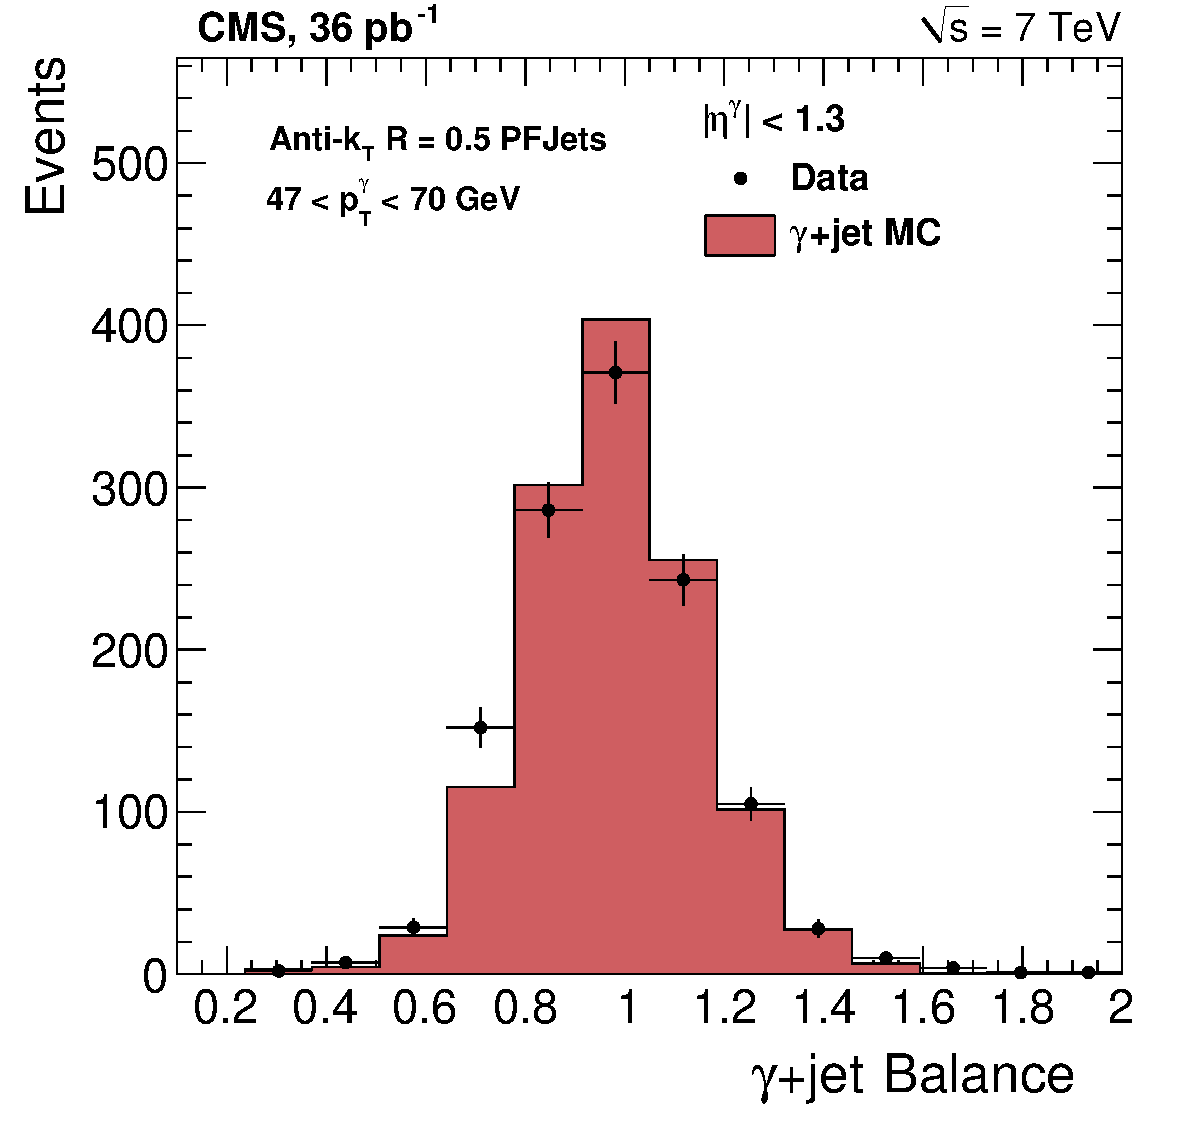
\includegraphics[width=0.45\textwidth]{Figures/JEC/response_L2L3_eta013_ptPhot_47_70}
    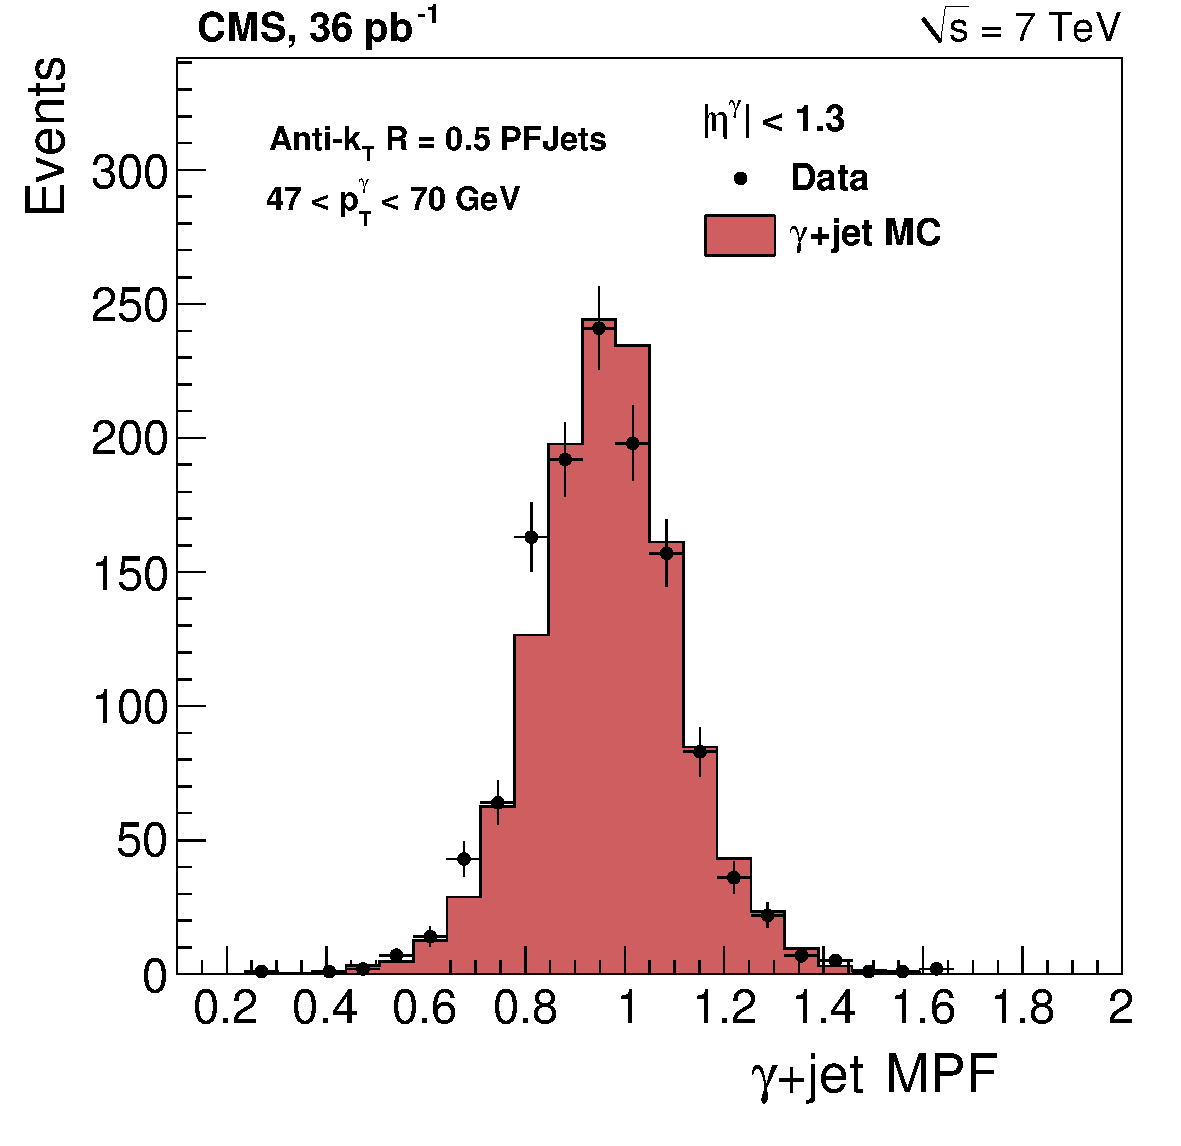
\includegraphics[width=0.45\textwidth]{Figures/JEC/responseMPF_eta013_ptPhot_47_70}
    \caption{Example response distributions for PF jets from \pt-balancing (left) and MPF (right) in the $\gamma$+jets sample.}
    \label{fig:photonResponse}
  \end{center}
\end{figure}

In the selected $\gamma$+jets sample, the presence of a barrel jet ($|\eta|<1.3$) recoiling against the photon candidate in azimuth by $\Delta \phi > 2.7$ is required. To reduce the effect of initial and final state gluon radiation that degrades the jet-photon \pt-balance, events containing additional jets with $\ptsecond > \alpha\cdot\pt^{\gamma}$ and outside the $\DeltaR=0.25$ cone around the photon direction are vetoed. The \pt-balance and MPF response measurements are performed in the same way with data and MC samples with different values of the threshold on $\alpha$ and the data/MC ratio is extrapolated to $\alpha=0$. This procedure allows the separation of the $\gamma$-jet intrinsic \pt-imbalance from the imbalance caused by hard radiation (Section~\ref{sec:radbias}). 

\begin{figure}[ht!]
  \begin{center}
    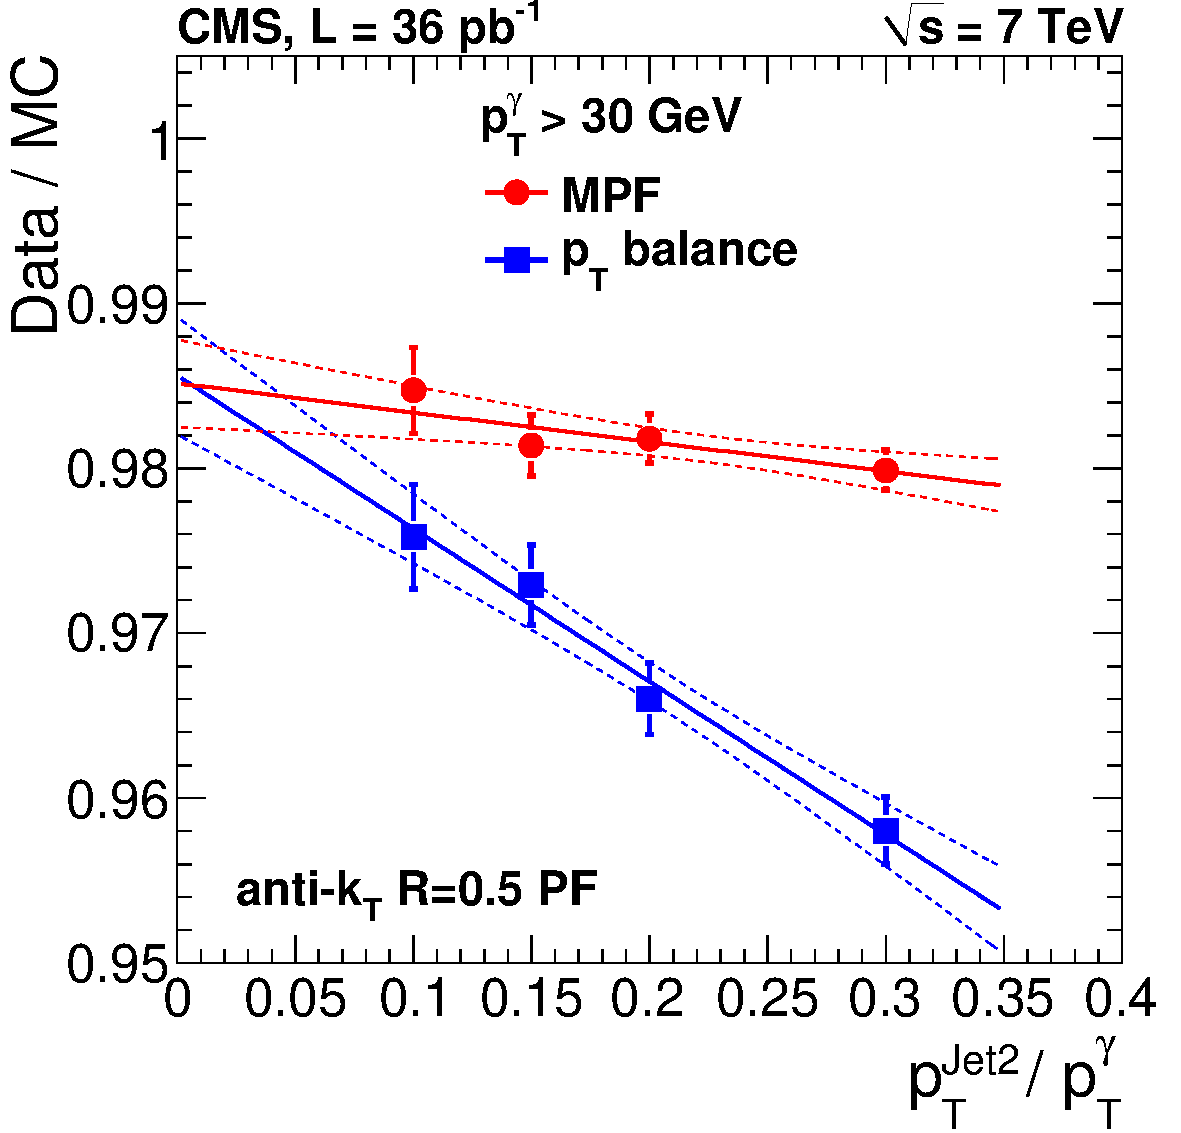
\includegraphics[width=0.45\textwidth]{Figures/JEC/MPF_pTbalance_vspT2nd_AK5}
    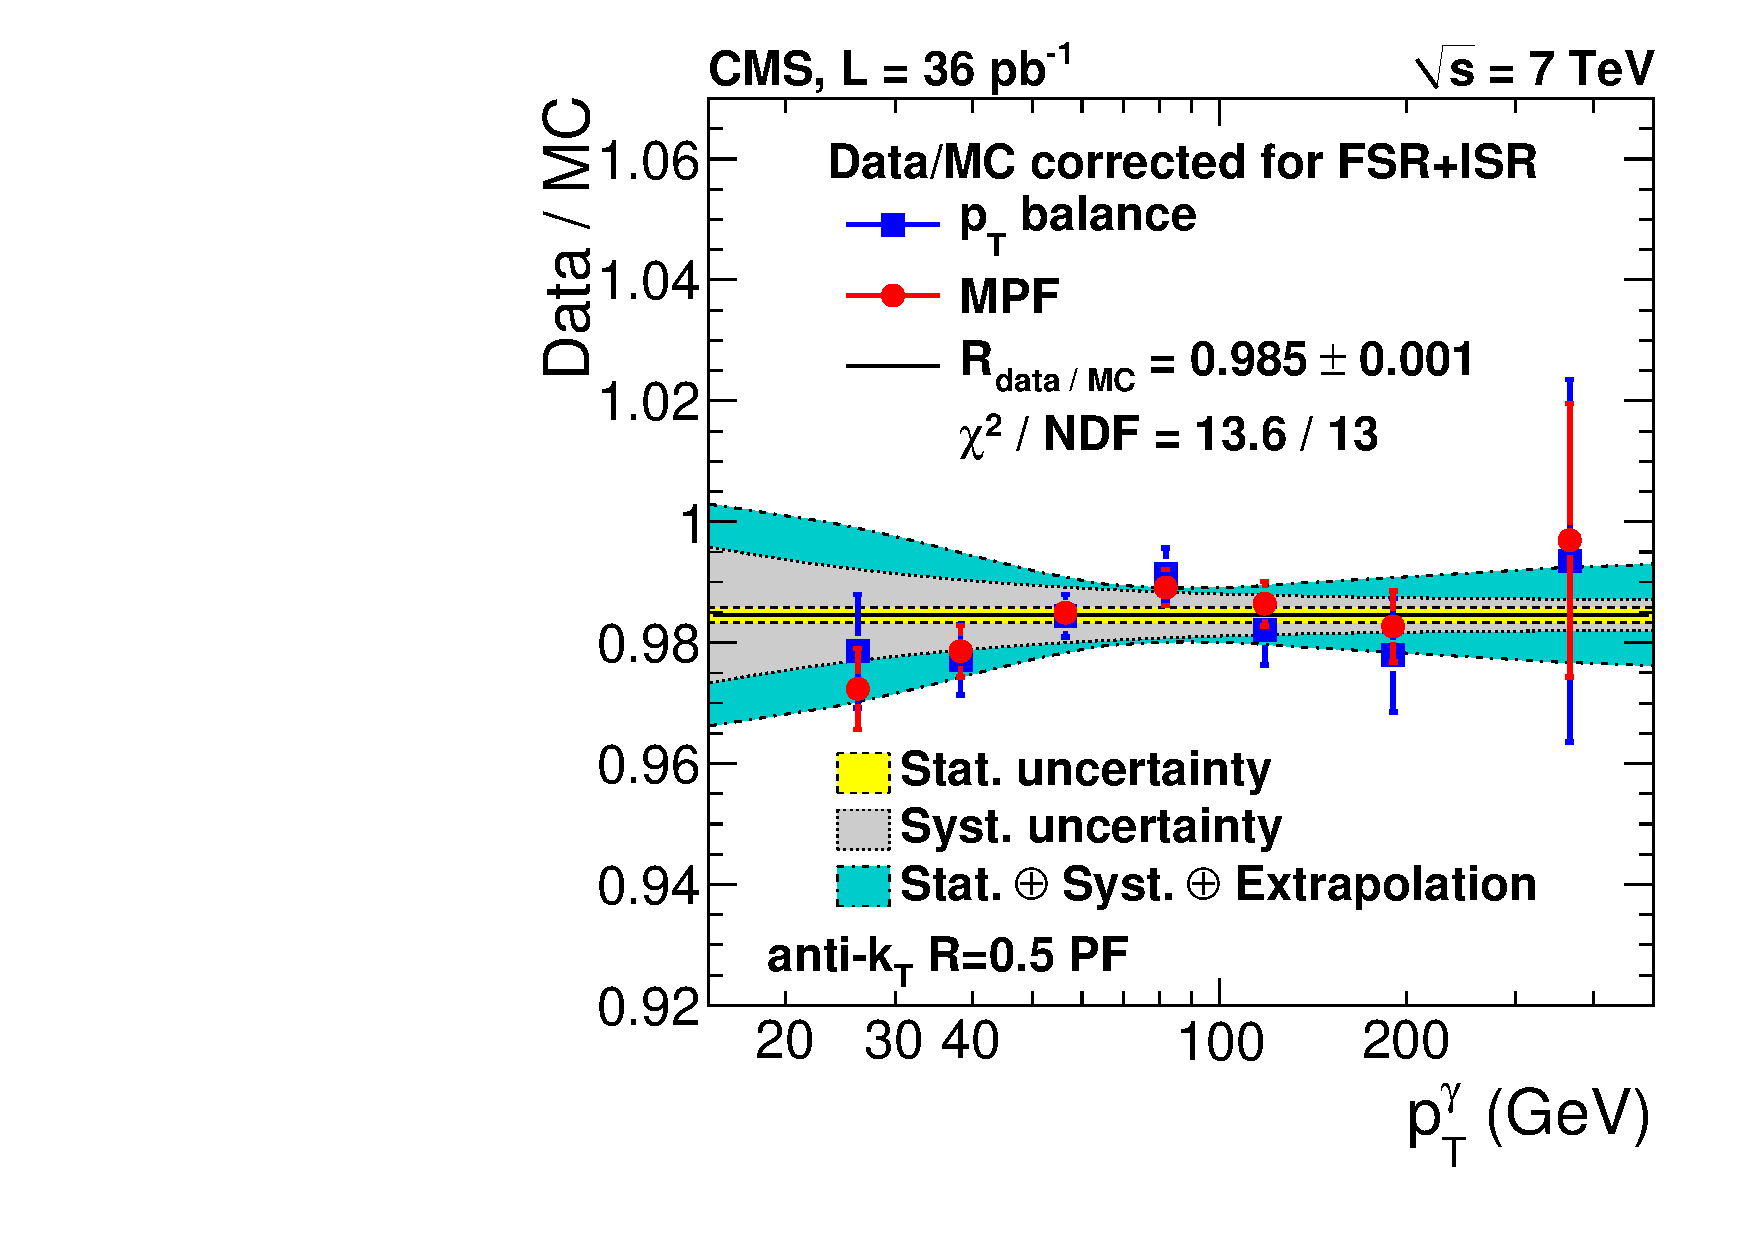
\includegraphics[width=0.45\textwidth]{Figures/JEC/FinalDataOverMC3_AK5}
    \caption{Left: dependence of the data/MC ratio of the jet energy response on the second jet \pt threshold. Right: data/MC ratio of the jet energy response, after extrapolation to zero second jet \pt, as a function of $\pt^\gamma$. Solid squares and solid circles correspond to the \pt-balancing and the MPF methods, respectively.}
    \label{fig:photon}
  \end{center}
\end{figure}

Figure~\ref{fig:photon} (left) shows the data/MC jet-energy-response ratio, relative to the $\gamma$ ECAL scale, extrapolated as a function of the threshold on the second jet \pt. In the \pt-balancing method, the secondary jet effect is more pronounced because it affects directly the transverse momentum balance between the photon and the leading jet. In the MPF method, the presence of the secondary jet(s) affects the measurement to a lesser extent, and mainly through the response difference between the leading jet and the secondary softer jet(s). For loose veto values, the ratio data/MC in both methods is lower than unity, while the agreement improves by tightening the veto. Figure~\ref{fig:photon} (right) shows the data/MC response ratio after the extrapolation to $\alpha=0$ for both MPF and \pt-balancing methods, as a function of $\pt^{\gamma}$. The two measurements are statistically uncorrelated to a good approximation and the two sets of points are fitted together with a constant value. The fit gives data/MC = $0.985 \pm 0.001$, relative to the $\gamma$ ECAL scale, which leads to an absolute response residual correction $C_\text{abs}=1/0.985=1.015$ (Eq.~(\ref{eq:jec_components})), constant in \pt.  

In addition to the $\gamma$+jets sample, the absolute jet energy response is also measured from the Z+jets sample. Figure~\ref{fig:ZJB} shows two characteristic response distributions in the $30\GeV<\pt^Z<60\GeV$ bin, as an example, measured from the $Z(\mu^+\mu^-)$+jets sample with the \pt-balancing and the MPF methods. The Z+jets samples cover the $\pt^Z$ range from 20\GeV to 200\GeV. 

\begin{figure}[ht!]
  \begin{center}
    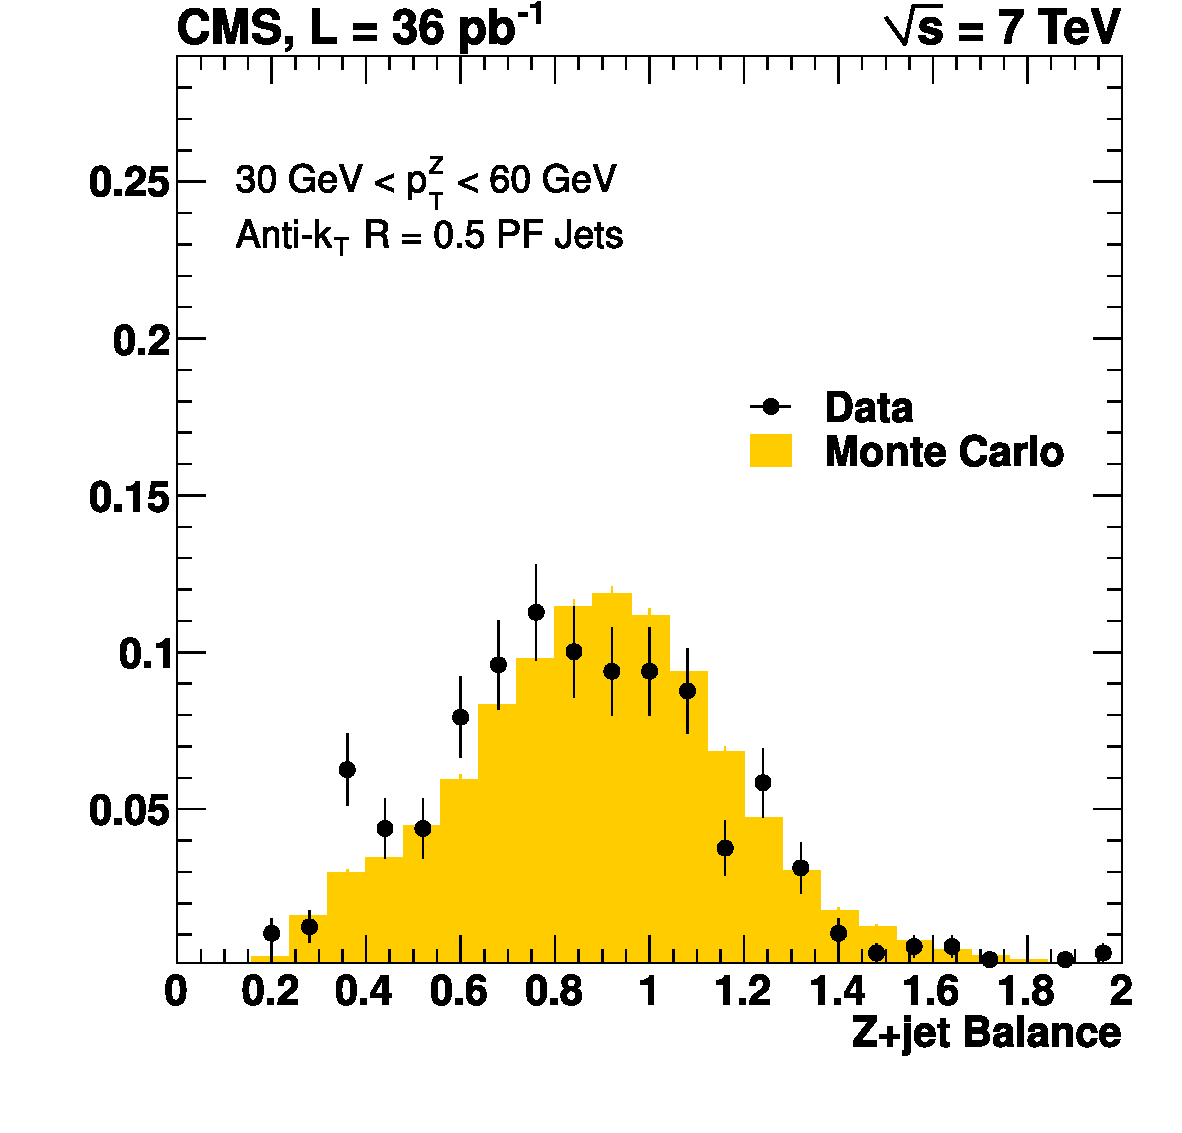
\includegraphics[width=0.45\textwidth]{Figures/JEC/jetresp_Pt30to60}
    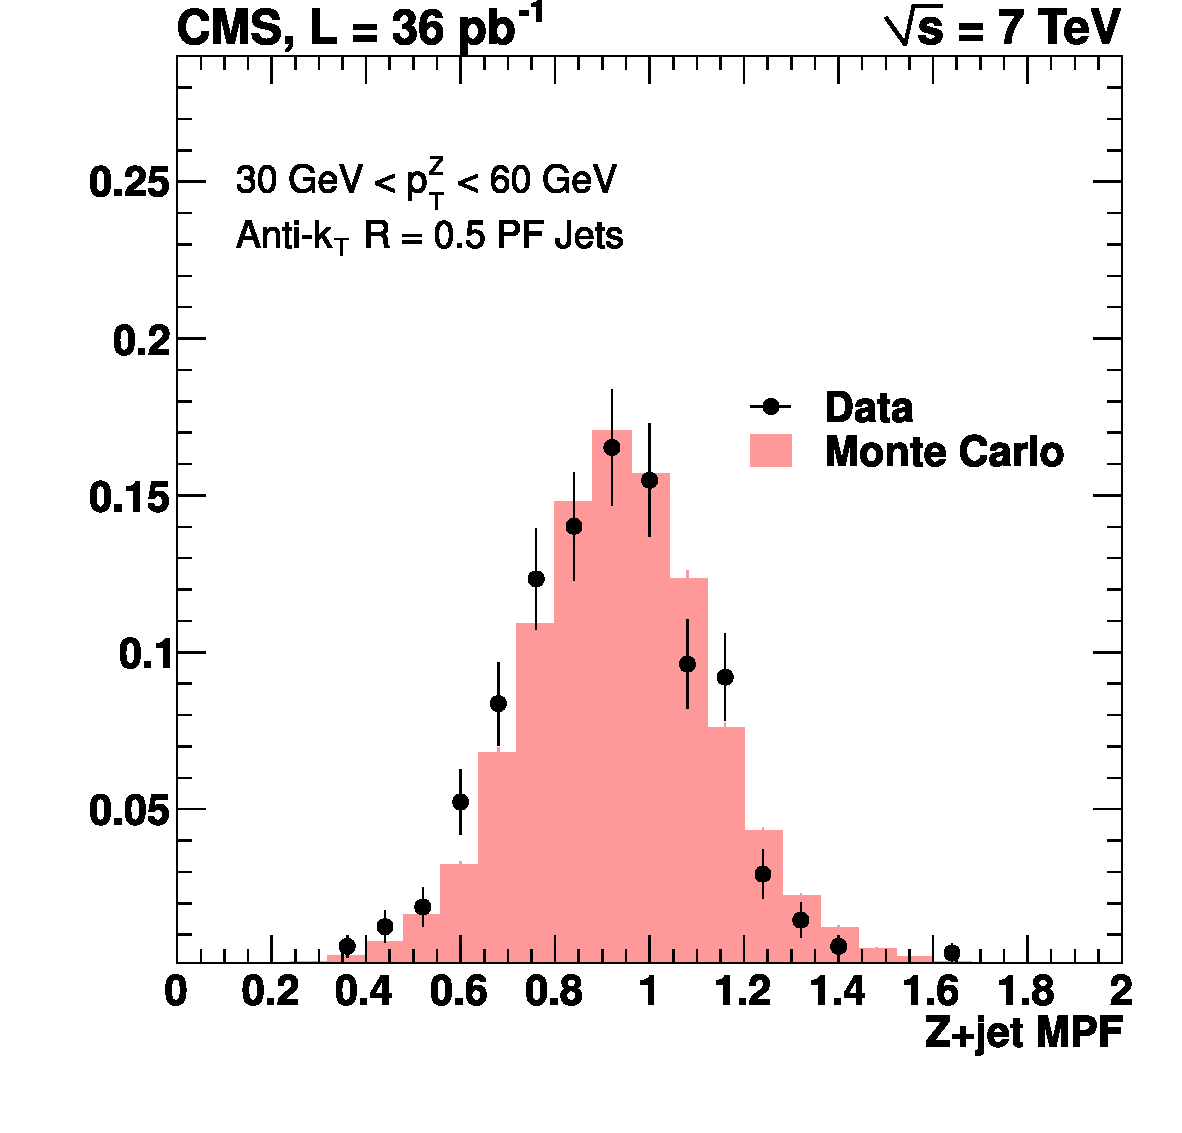
\includegraphics[width=0.45\textwidth]{Figures/JEC/mpfresp_Pt30to60}
    \caption{Left: jet energy response from $Z(\mu^+\mu^-)$+jets \pt-balancing in the bin $30<\pt^Z<60\GeV$. Right: jet energy response from $Z(\mu^+\mu^-)$+jets MPF in the bin $30<\pt^Z<60\GeV$.}
    \label{fig:ZJB}
  \end{center}
\end{figure}

\begin{figure}[ht!]
  \begin{center}
    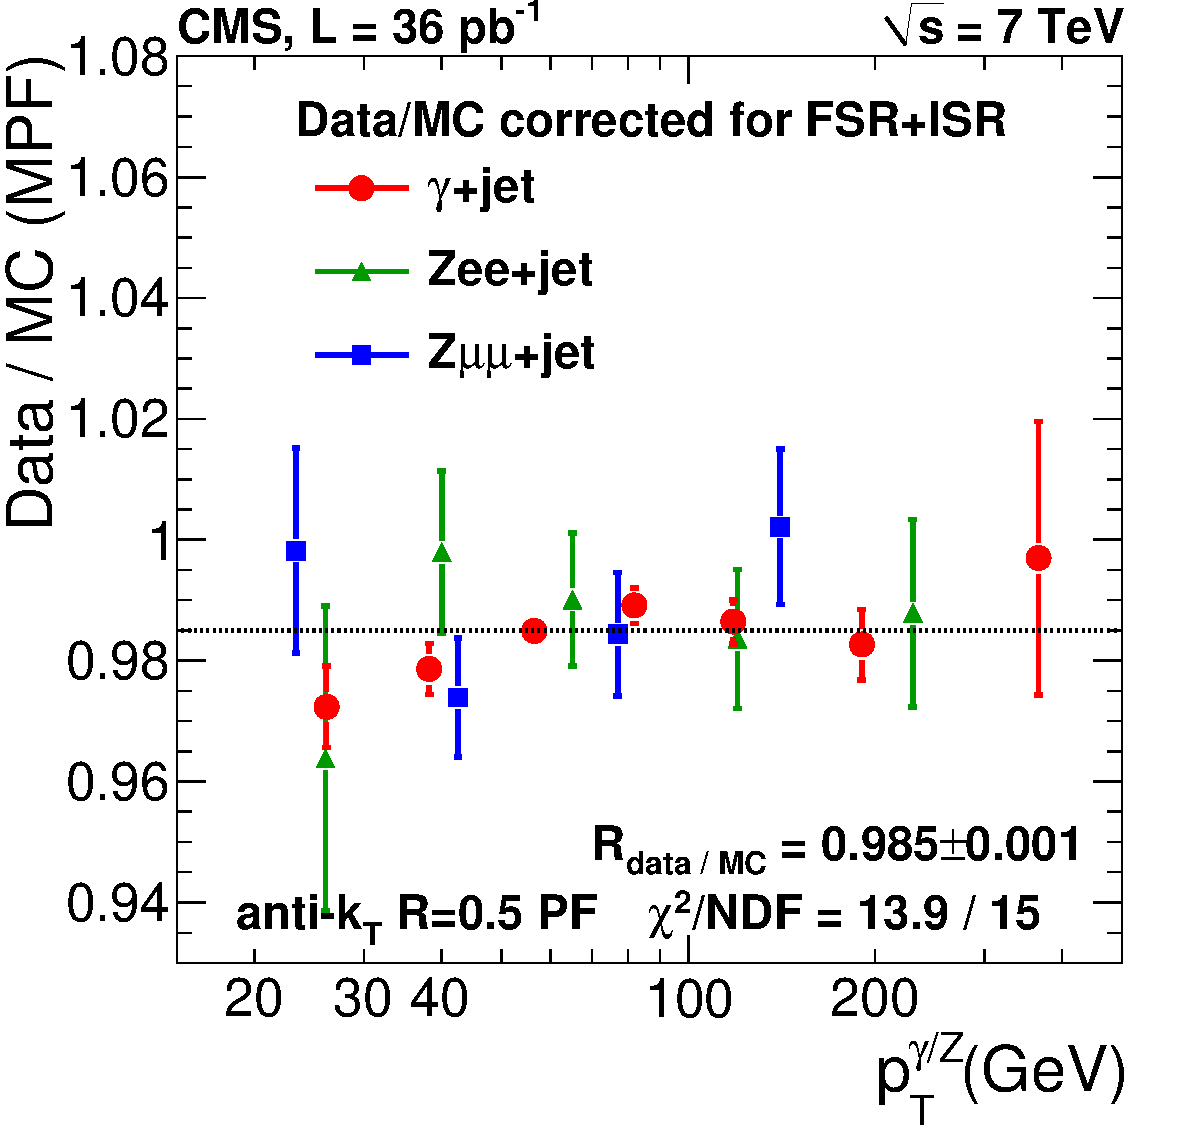
\includegraphics[width=0.45\textwidth]{Figures/JEC/FinalDataOverMC4_plusZ_AK5}
    \caption{Ratio of data over MC for the MPF response, as a function of $\pt^{\gamma,Z}$ in the photon+jet sample (circles), $Z(e^+e^-)$+jet sample (triangles) and $Z(\mu^+\mu^-)$+jet sample (squares).}
    \label{fig:dataMCAll}
  \end{center}
\end{figure}

In order to combine the results from the photon+jet and Z+jet samples, the more precise MPF method is employed identically in all relevant samples. Figure~\ref{fig:dataMCAll} shows the data/MC ratio as a function of $\pt^{\gamma,Z}$ after correcting for the final and initial state radiation differences between data and simulation (extrapolation to $\alpha=0$). Although the size of the Z+jets data sample is smaller than the $\gamma$+jets sample, the results from all samples are in good agreement, within the corresponding statistical uncertainties.

\subsubsection{Uncertainty Sources}

The uncertainty of the absolute jet energy scale measurement has six components: uncertainty in the MPF method for PF jets, photon energy scale, MC extrapolation beyond the reach of the available dataset, offset due to noise and pile-up at low-\pt (as discussed in Section~\ref{sec:offset_unc}), MC residuals (the level of closure of the MC correction in the MC), and the jet-by-jet matching residuals for CALO and JPT jets.  

{\bf MPF Uncertainty for PF Jets.} The MPF method is affected by several small uncertainties that mainly contribute at low \pt: flavour mapping, parton-to-particle level sensitivity, QCD background, secondary jets, and proton fragments. The various contributions are shown in Fig.~\ref{fig:jecuncert_mpf}.

\begin{figure}[ht!]
  \begin{center}
    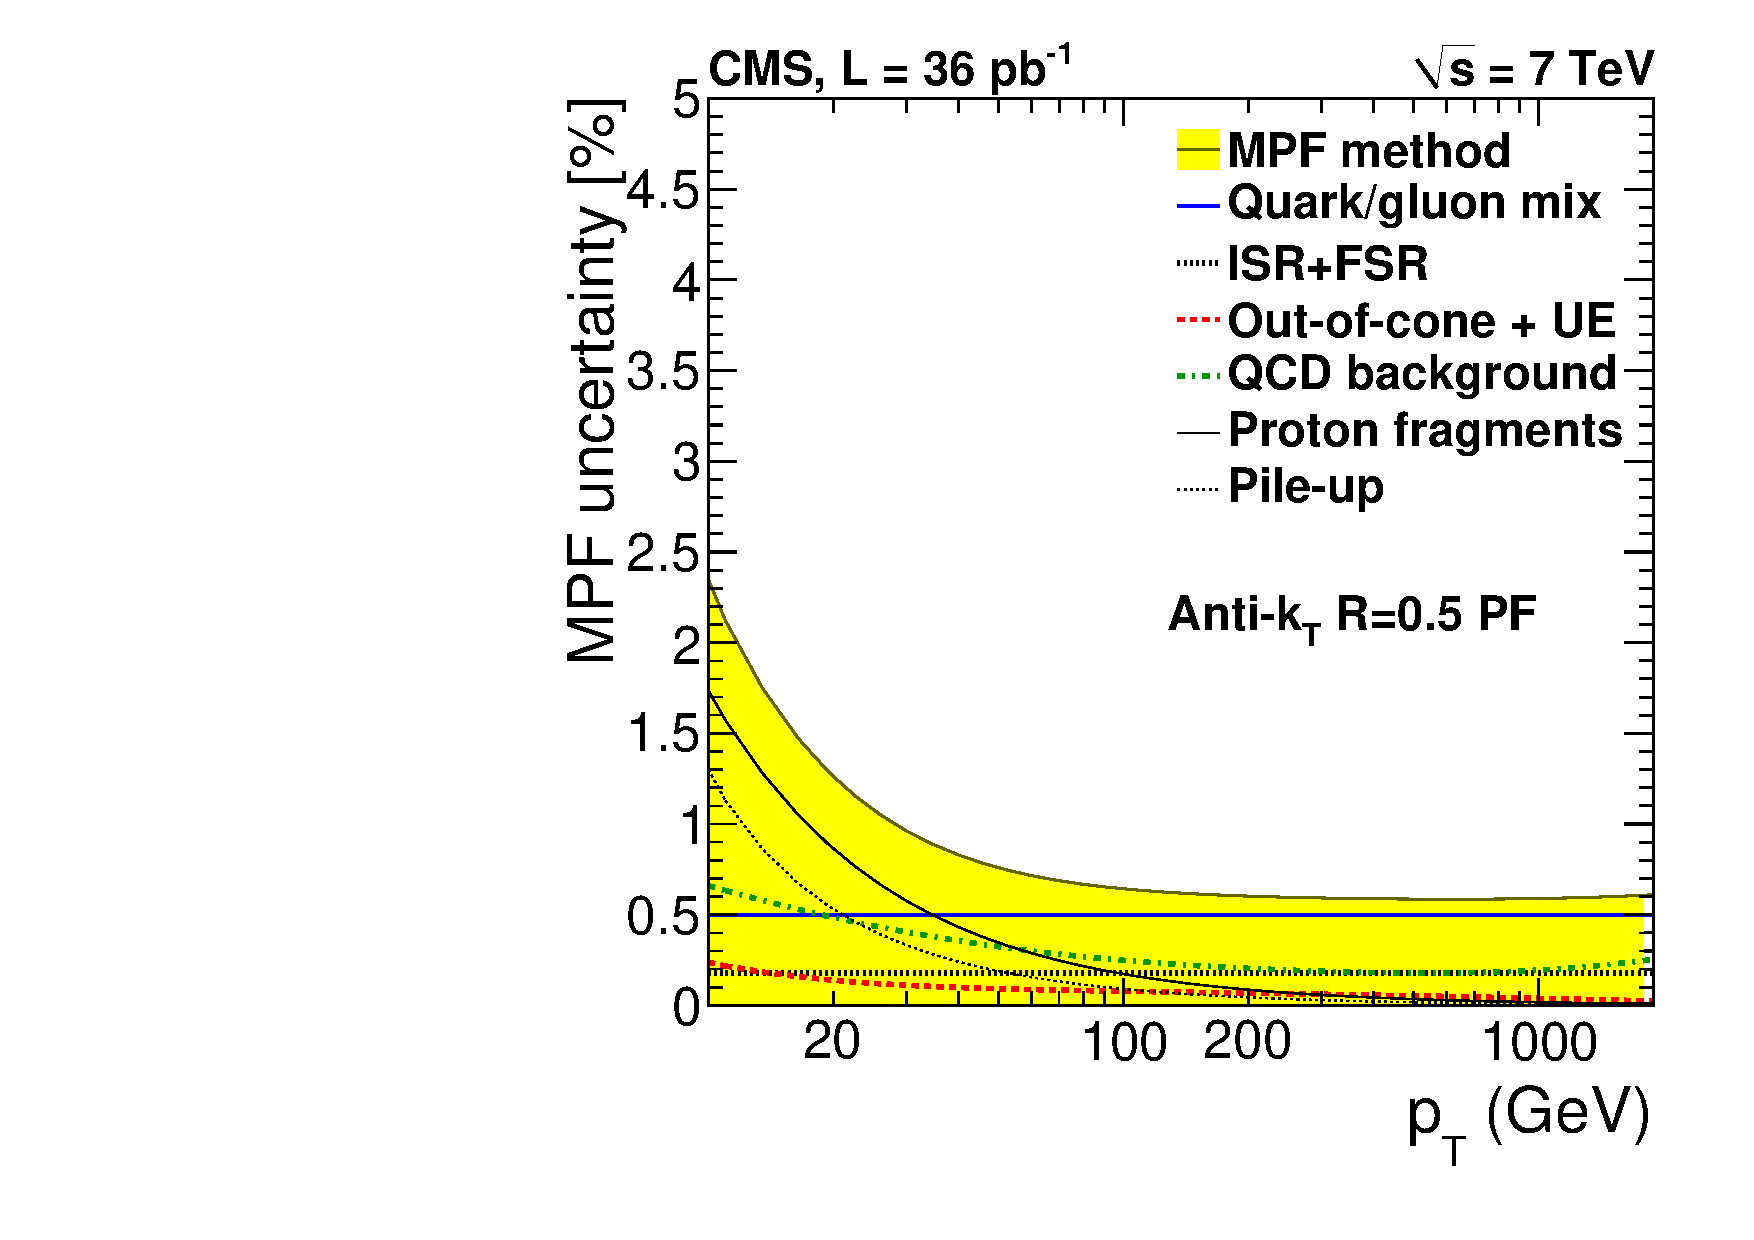
\includegraphics[width=0.45\textwidth]{Figures/JEC/JECUncert_MPF}
    \caption{Jet energy scale uncertainty in the MPF method for PF jets.}
    \label{fig:jecuncert_mpf}
  \end{center}
\end{figure}

The flavour mapping uncertainty accounts for the response difference between jets in the quark-rich $\gamma$+jets sample used to measure the absolute jet energy scale, and those in the reference, gluon-rich QCD multijet sample. This is estimated from the average quark-gluon response difference between {\sc PYTHIA6} and {\sc Herwig++} (Fig.~\ref{fig:flavor_herwigpythia}) in the region $30-150\GeV$. The latter is chosen because it is the \pt region best constrained by the available data. For PF jets, the flavour mapping uncertainty amounts to $\sim 0.5\%$.

By definition, the MPF response refers to the parton level because the photon is perfectly balanced in the transverse plane, against the outgoing partons. However, the default jet energy response refers to the particle level, which includes the UE and the hadronization effects. The parton-to-particle level response interpretation therefore is sensitive to the UE and the out-of-cone showering (OOC). The corresponding uncertainty is estimated from the simulation by using jets reconstructed with larger size parameter ($R=0.7$, more sensitive to UE and OOC) and comparing the extrapolation to the zero secondary jet activity with respect to the nominal size parameter ($R=0.5$). The resulting uncertainty has a weak \pt-dependence and is smaller than $0.2\%$. 

The dominant background for $\gamma$+jets events is the QCD dijet production where one leading jet fragments into a hard isolated $\pi^0\to\gamma+\gamma$. Such events can alter the measured \pt-balance because the leading neutral $\pi^0$ carries only a fraction of the initial parton energy. The QCD background uncertainty is estimated by repeating the measurement, using a loose and a tight photon identification, and is found to be negligible compared to the current statistical precision.

The MPF response at low \pt is sensitive to the undetected energy that leaks outside the forward calorimeter acceptance at $|\eta|>5$ (proton fragments). This results in an underestimation of the MPF response, compared to the true response. The uncertainty due to the undetected energy is taken from the simulation and is estimated to be $50\%$ of the difference between the MPF response and the true response. 

The secondary jet activity is found to be significantly different between data and MC, and it is corrected by extrapolating the data/MC ratio for the MPF and \pt-balance methods to zero secondary jet activity. The related uncertainty is estimated as half of the radiation bias correction applied to the MPF method.

{\bf Photon Energy Scale Uncertainty.} The MPF and \pt-balancing methods are directly sensitive to the uncertainty in the energy of the $\gamma$ used as a reference object. The $\gamma$ energy scale uncertainty is estimated to be $\sim 1\%$ based on studies presented elsewhere~\cite{EGM-10-003}.

{\bf Monte Carlo Extrapolation.} The in situ measurement of the absolute jet energy scale is feasible only in the \pt range where $\gamma$+jets data are available. For the current dataset this range extends to around $300\GeV$. However, the jet \pt range probed in the entire dataset is generally more than three times higher than in the $\gamma$+jets sample. In QCD dijet events, jets as high as $\pt = 1\TeV$ are observed. Because of the absence of data for direct response measurement at high \pt, the calibration relies on the simulation. Based on the data vs. MC comparison in the region of available $\gamma$+jets data, conclusions can be drawn for the extrapolation of the jet energy correction at the highest jet \pt.

\begin{figure}[ht!]
  \begin{center}
    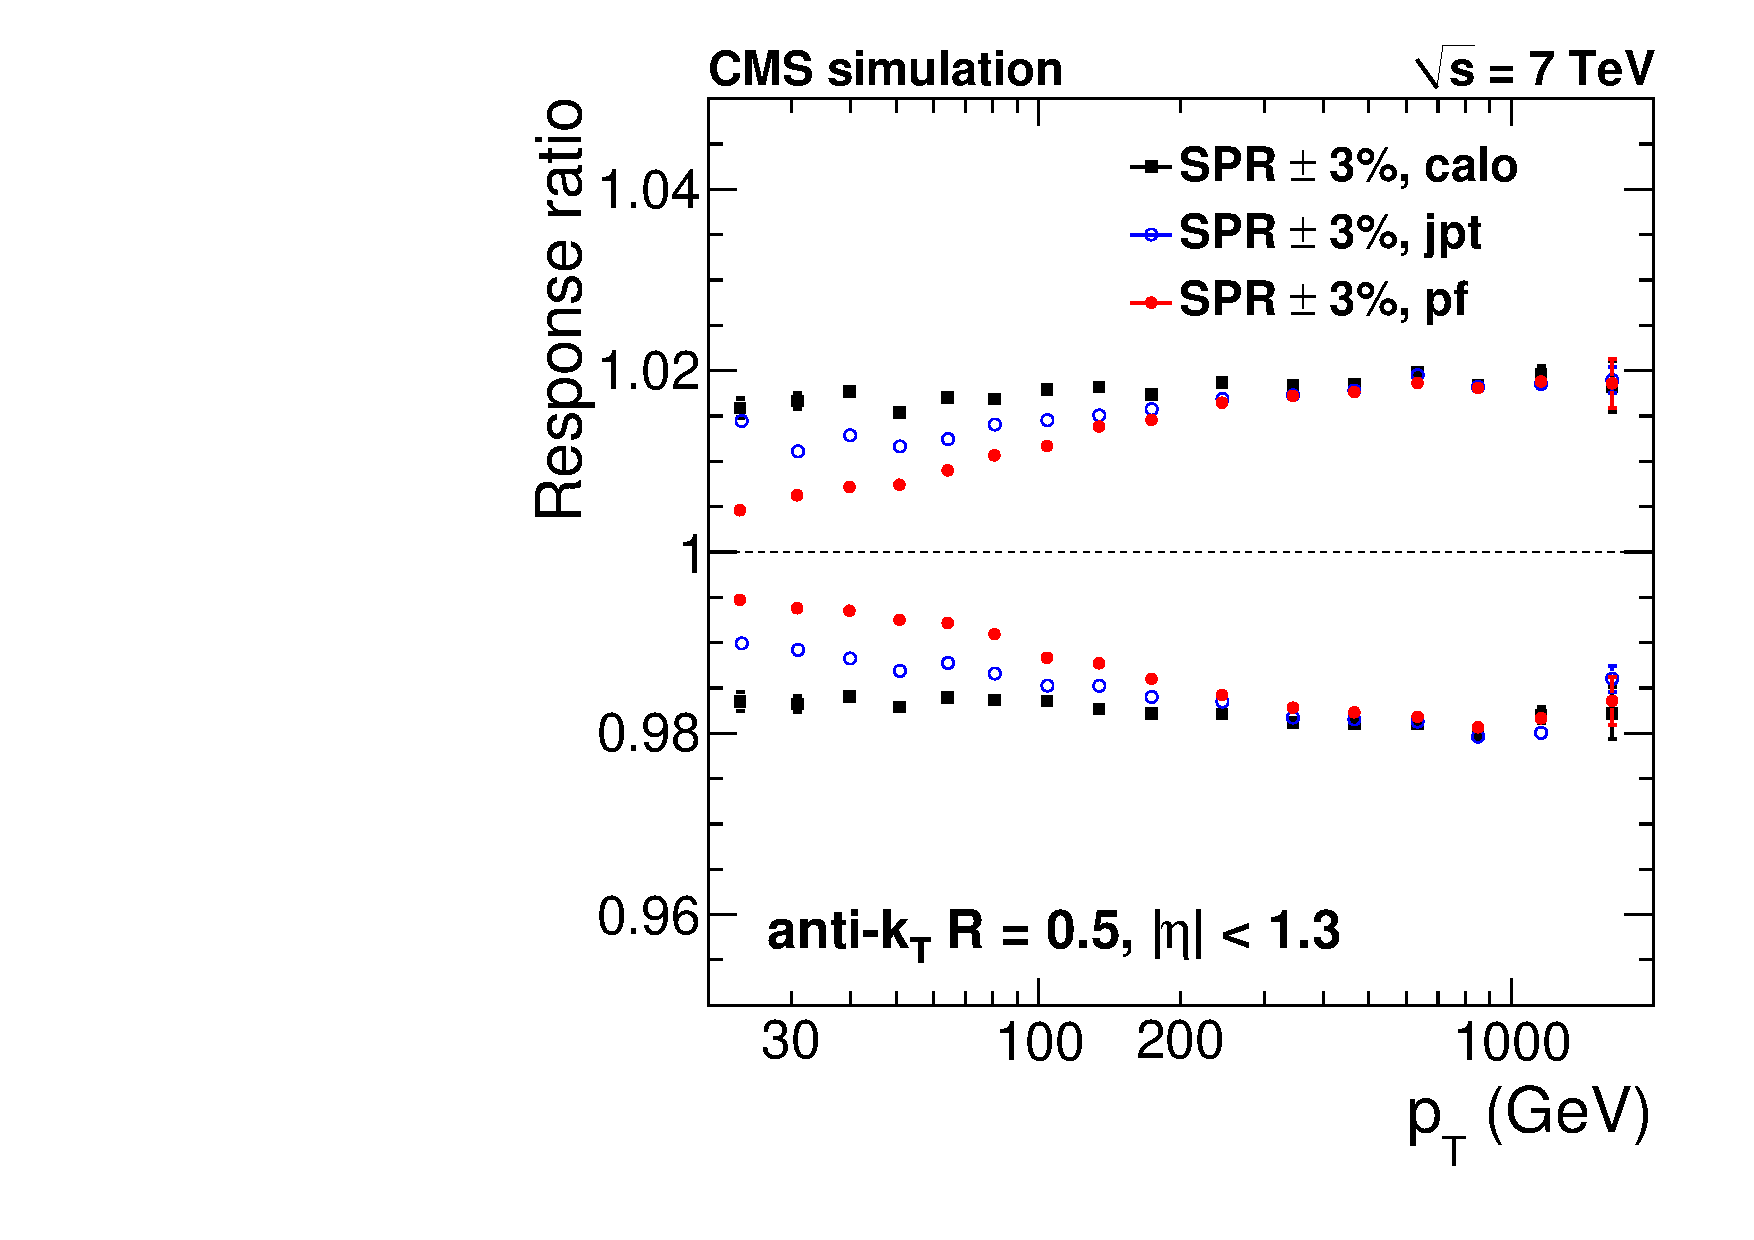
\includegraphics[width=0.45\textwidth]{Figures/JEC/singlepionresponse} 
    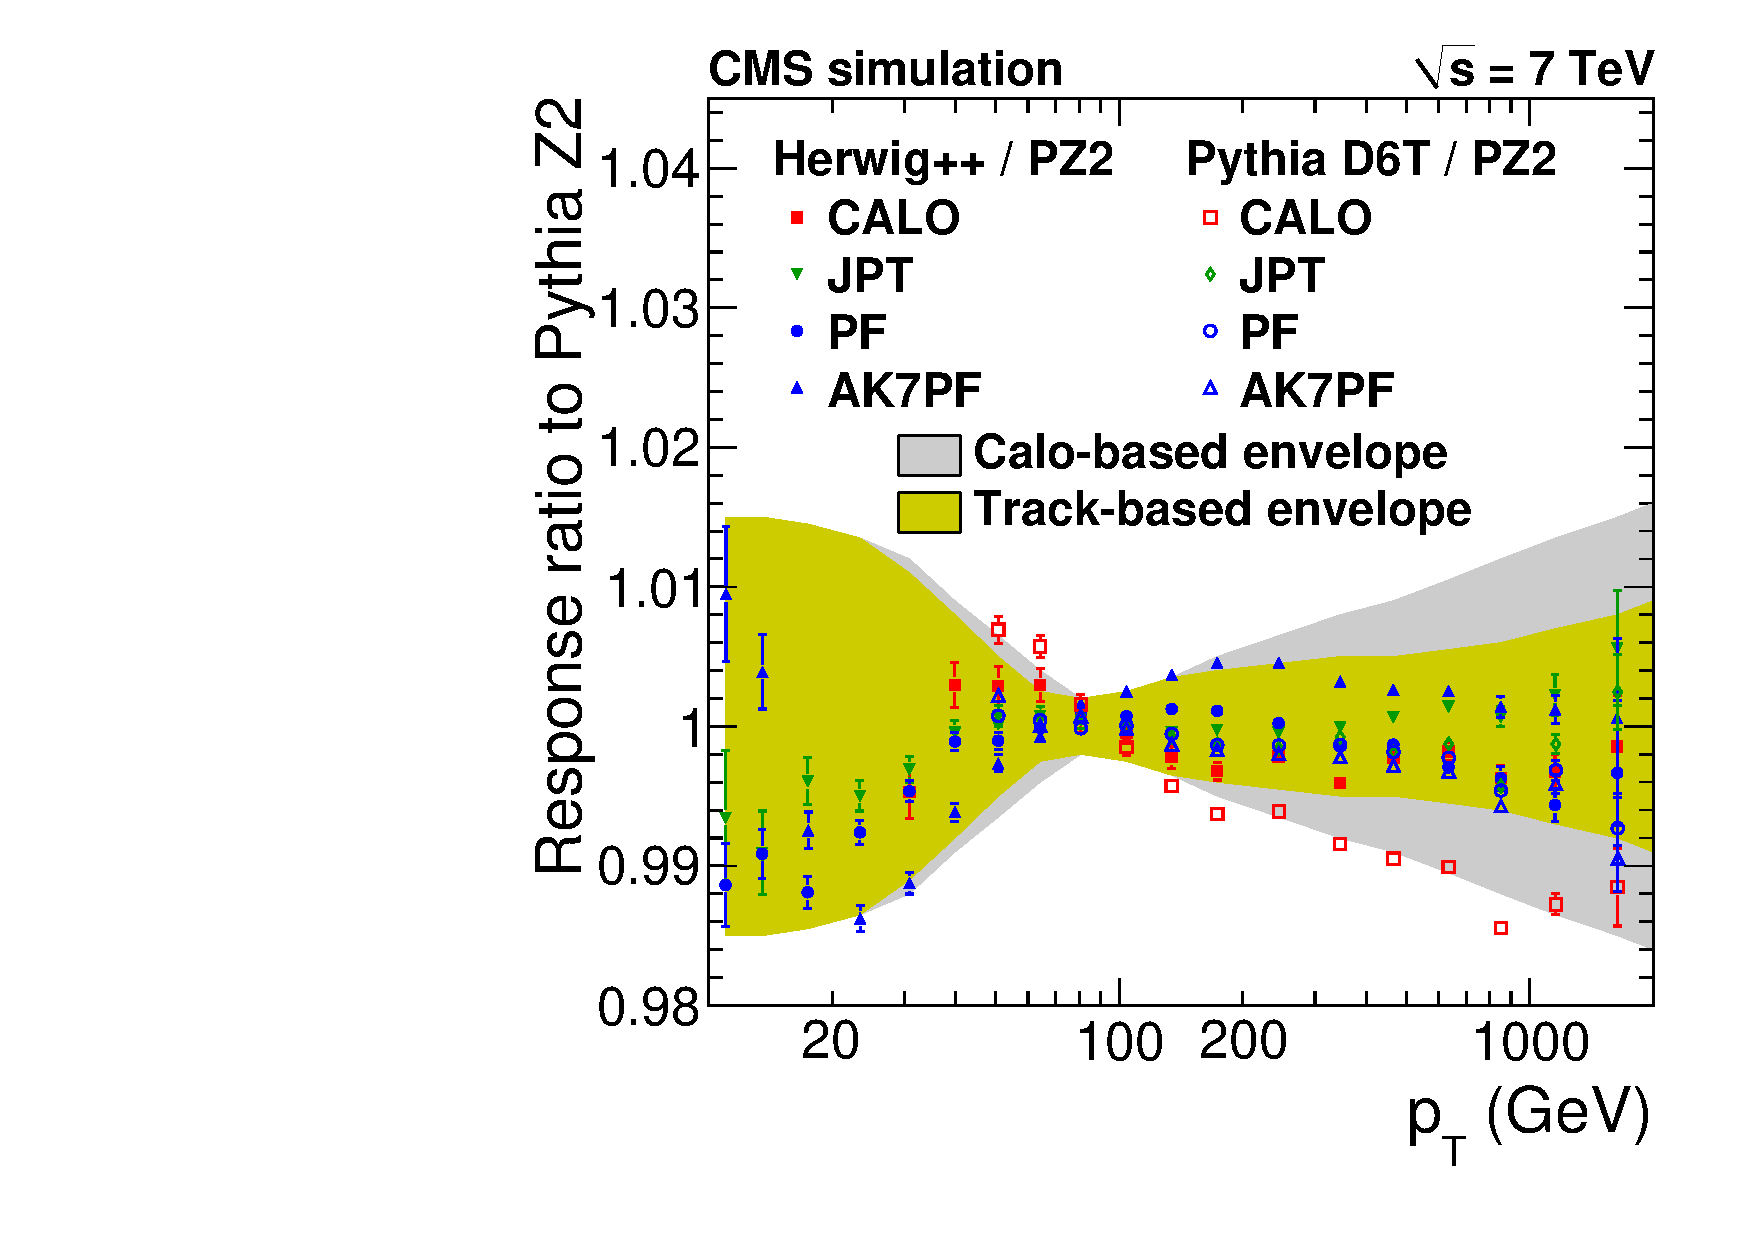
\includegraphics[width=0.45\textwidth]{Figures/JEC/highpt_envelope}
    \caption{Left: sensitivity of the jet energy response in $|\eta|<1.3$ to the single-particle response (SPR) uncertainty. Right: dependence of the jet energy response on the fragmentation model. Here AK7PF stands for PF jets reconstructed with the anti-$k_T$ algorithm with size parameter $R=0.7$.}
    \label{fig:FragSpr}
  \end{center}
\end{figure}

The simulation uncertainty for the high-\pt jets arises from two main sources: the single-particle response (SPR) for hadrons and the fragmentation modeling. The former is measured directly in data by using isolated tracks and comparing the energy deposited in the calorimeters with the momentum measured by the tracker. The currently available measurement~\cite{JME-10-008} indicates that the data/MC disagreement is less than 3\%. The SPR uncertainty is translated to a jet energy response uncertainty by modifying accordingly the simulation. Figure~\ref{fig:FragSpr} (left) shows the impact of the SPR uncertainty on the response of the different jet types, in the region $|\eta|<1.3$. For CALO jets, the induced uncertainty is roughly constant vs. \pt and approximately equal to 2\%. The track-based algorithms are less affected at low-\pt by the SPR uncertainty because the energy is primarily measured by the tracker. However, as the jet \pt increases and the track momentum measurement becomes less precise compared to the calorimetric measurement, the track-based jet types behave like CALO jets. The transition is smooth and is completed at jet $\pt\sim 300\GeV$. 

The other source of systematic uncertainty is related to the fragmentation properties, which include the parton shower and the hadronization simulation. Since jets are composite objects, realized as ``sprays" of highly collimated particles, and the calorimeter response is non-linear, the jet energy response depends on the number and the spectrum of the particles it consists of. The sensitivity to the fragmentation modelling is studied by generating QCD events from various MC generators which are then processed by the full simulation of the CMS detector. The MC generators employed are: {\sc PYTHIA6} (tunes D6T~\cite{D6T} and Z2) and {\sc Herwig++}\cite{HERWIG}. Figure~\ref{fig:FragSpr} (right) shows the response ratio of the various models with respect to {\sc PYTHIA6},with Z2 tune, which is the default. The differences between the models are negligible at $\pt\sim 80\GeV$, while they grow up to 1.5\% at low and high jet \pt. 

The combined MC uncertainty of the absolute jet energy response due to SPR and fragmentation is shown in Fig.~\ref{fig:highptUnc}.

\begin{figure}[ht!]
  \begin{center}
    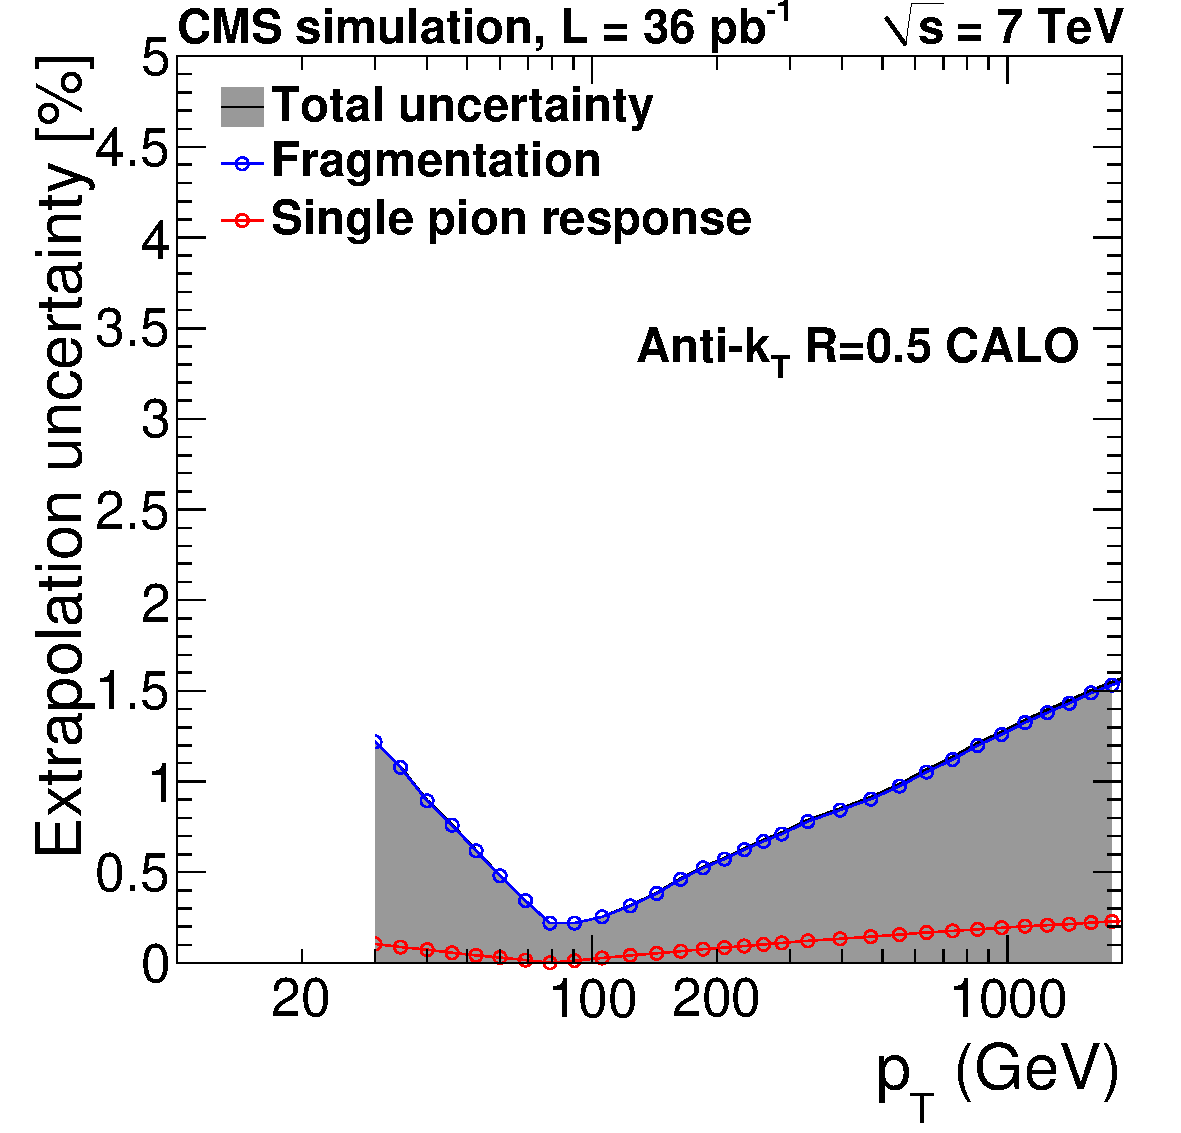
\includegraphics[width=0.45\textwidth]{Figures/JEC/JECUncert_HighPt_CALOAK5}
    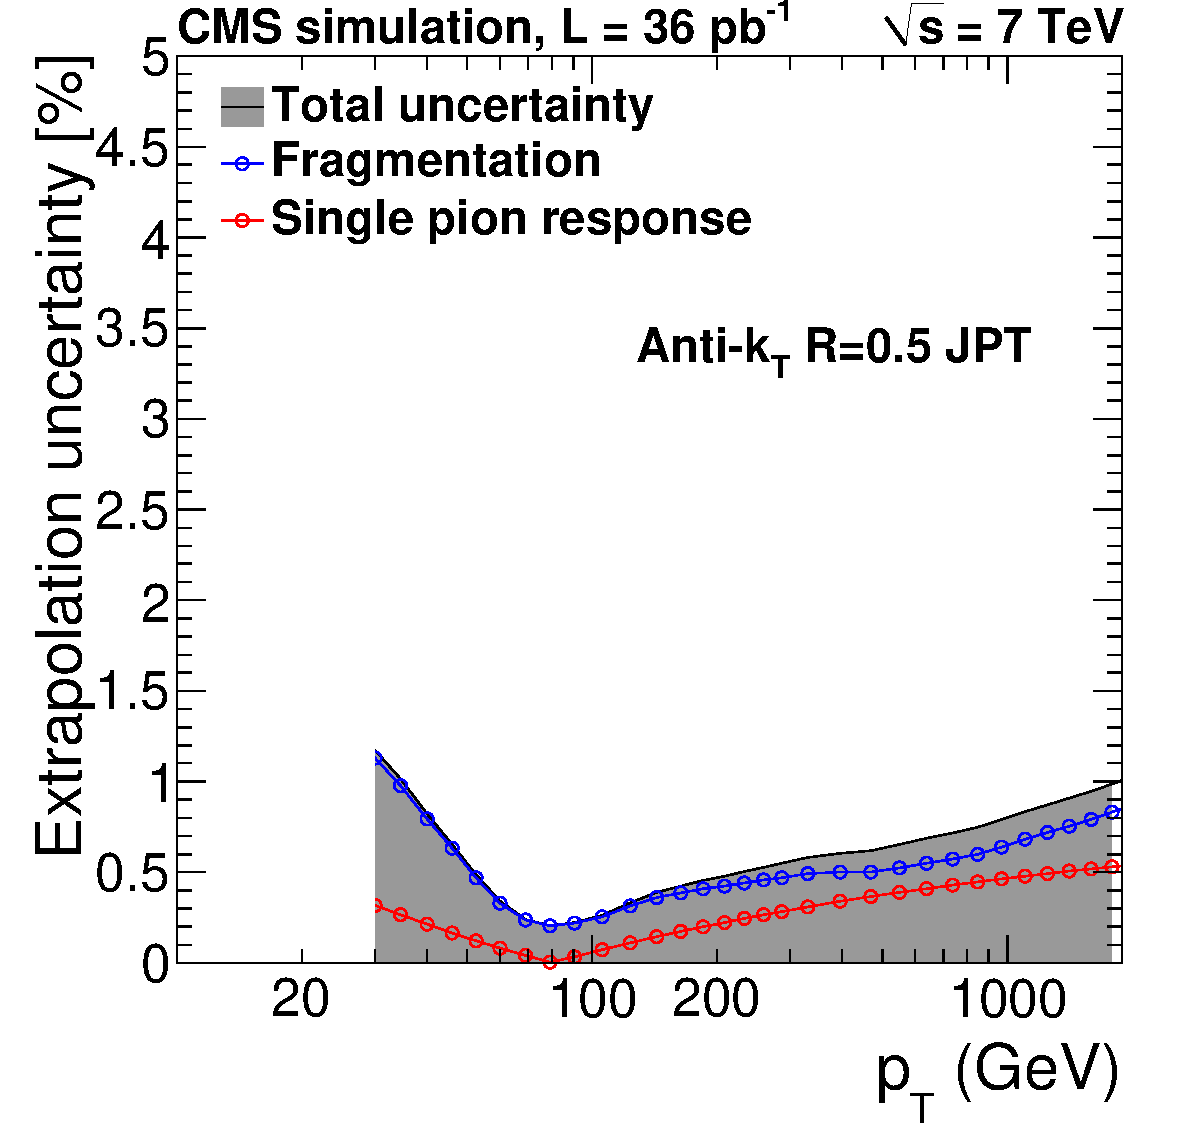
\includegraphics[width=0.45\textwidth]{Figures/JEC/JECUncert_HighPt_JPTAK5}
    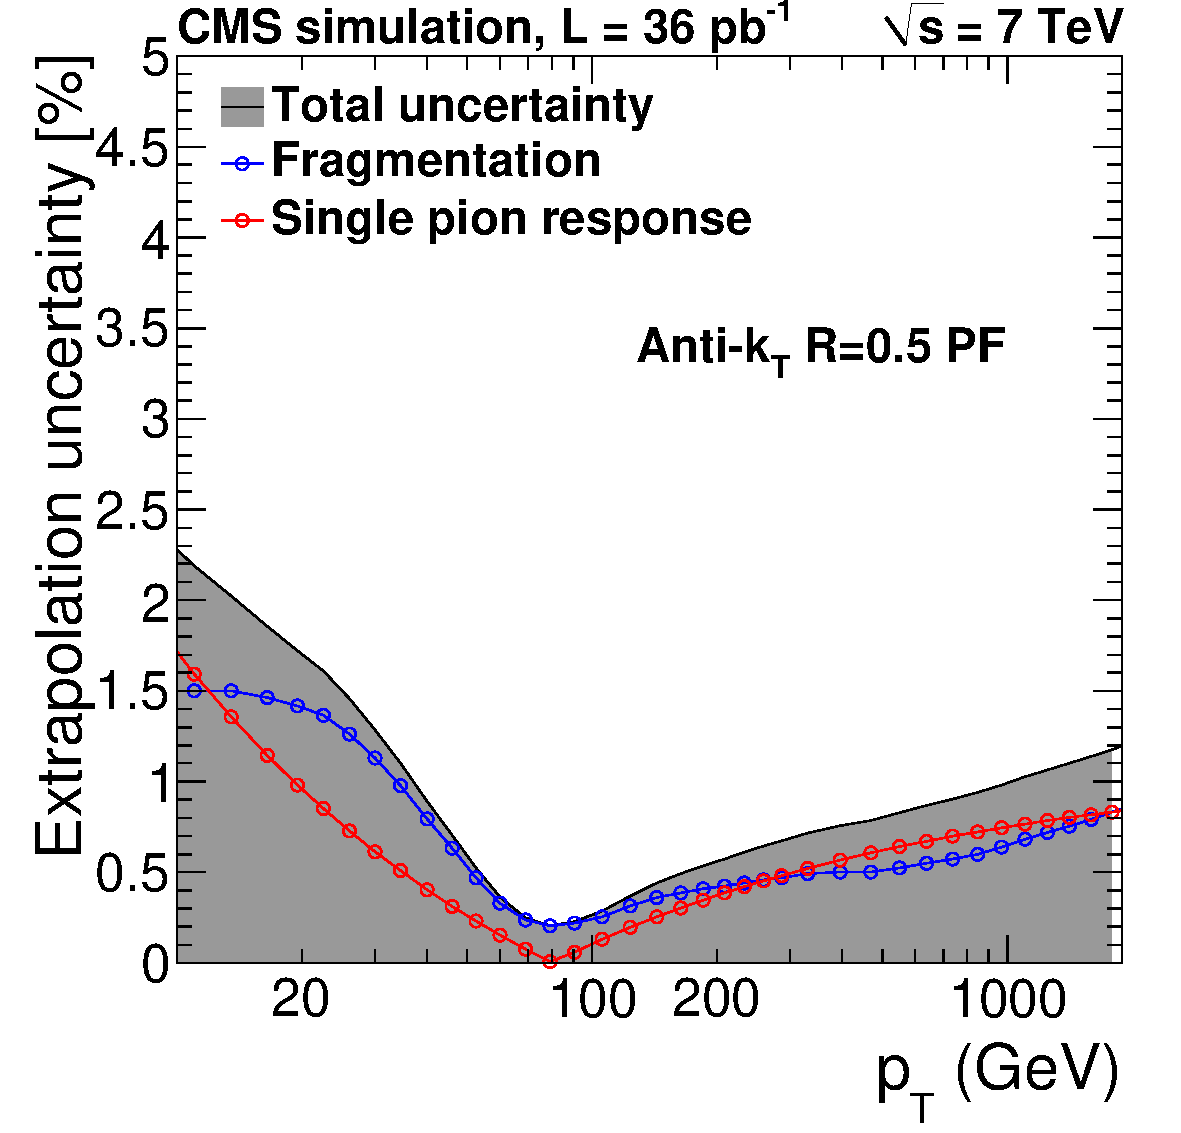
\includegraphics[width=0.45\textwidth]{Figures/JEC/JECUncert_HighPt_PFAK5}
    \caption{Uncertainty of the absolute jet energy response in the region $|\eta|<1.3$ related to the MC extrapolation for CALO, JPT and PF jets respectively. }
    \label{fig:highptUnc}
  \end{center}
\end{figure}

The particle-flow algorithm reconstructs individual particles, prior to jet clustering. This allows the detailed study of the PF jet composition in terms of charged hadrons, photons and neutral hadrons. In particular, the jet energy response is closely related to the energy fraction carried by the three major composition species. The purpose of this study is to demonstrate that the MC simulation is able to describe accurately the PF jet composition observed in data and therefore can be trusted to predict the PF jet response in the kinematic regions where the in situ measurement is not possible.

\begin{figure}[ht!]
  \begin{center}
    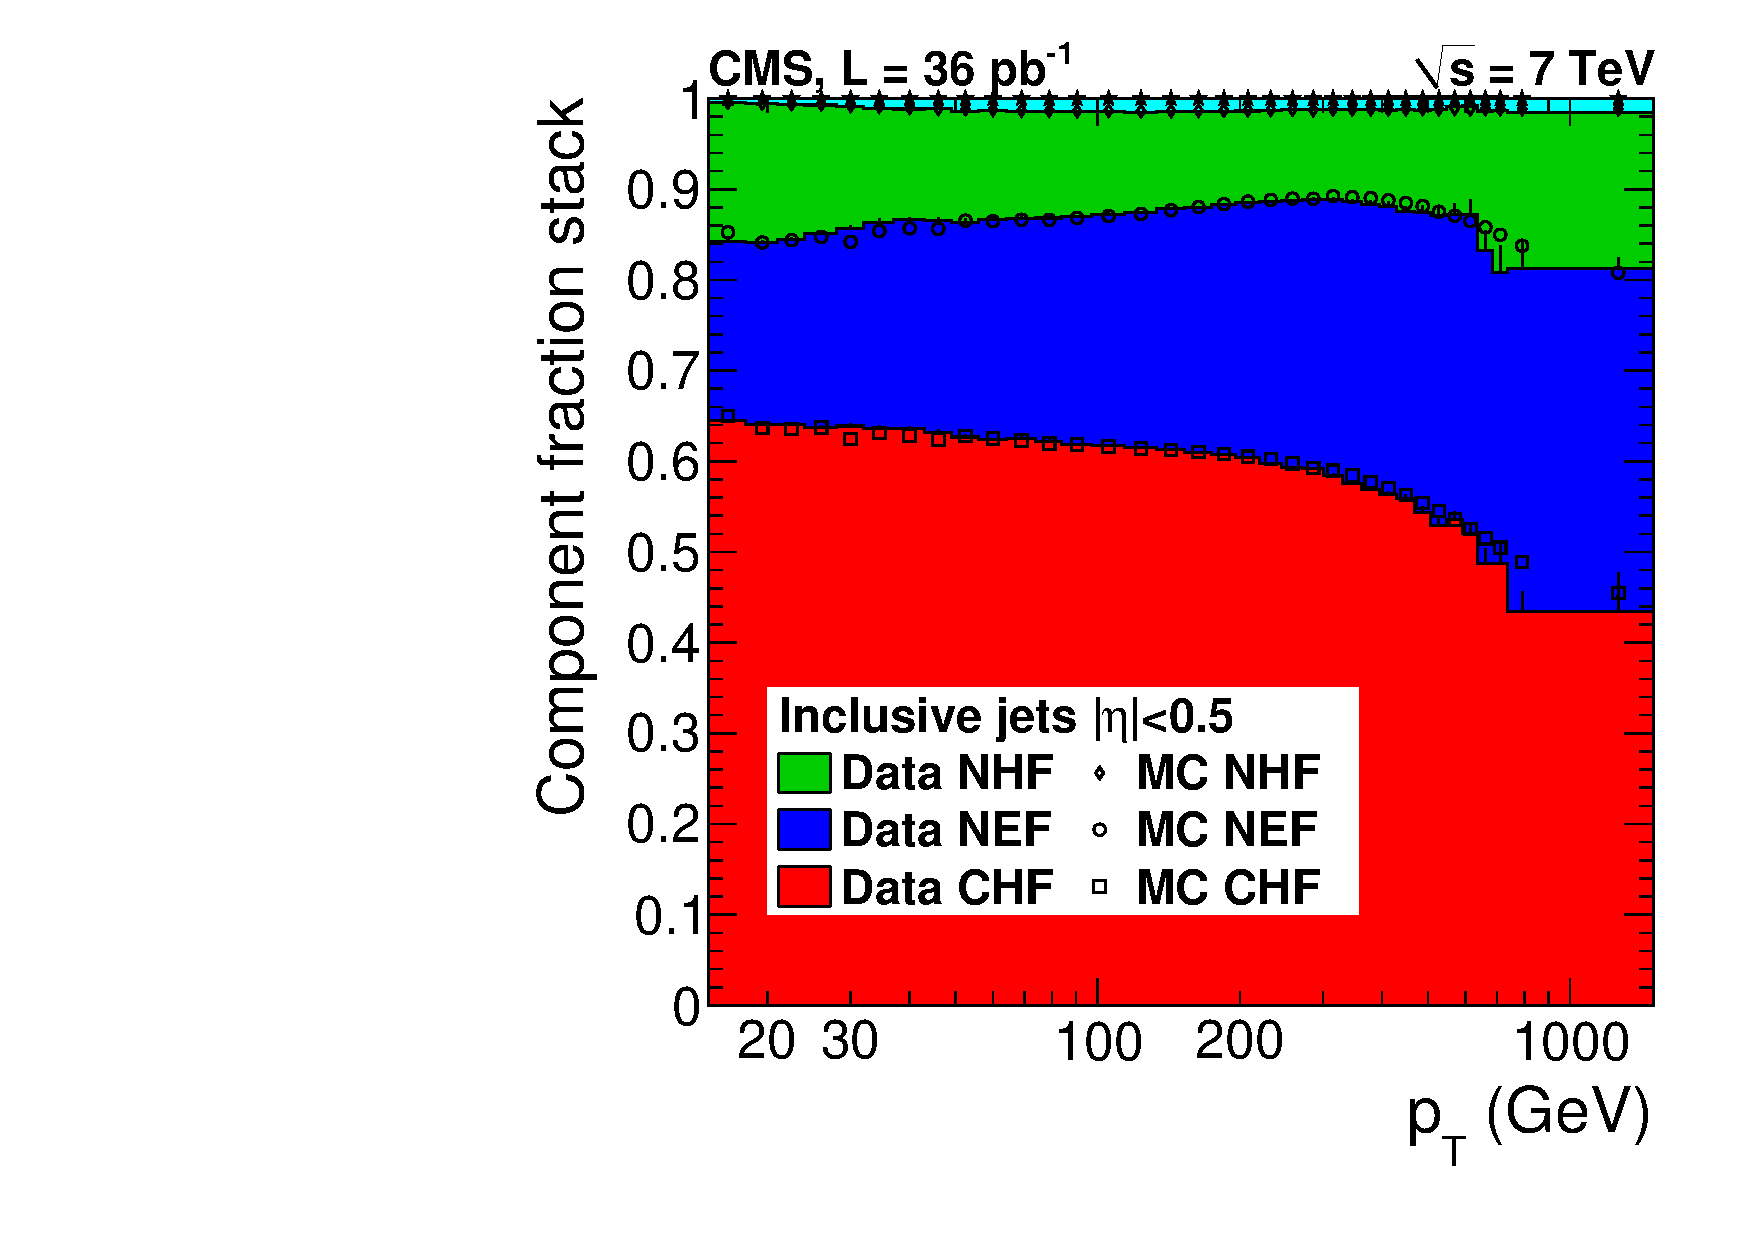
\includegraphics[width=0.45\textwidth]{Figures/JEC/jecChecks_fracstack_Rap0}
    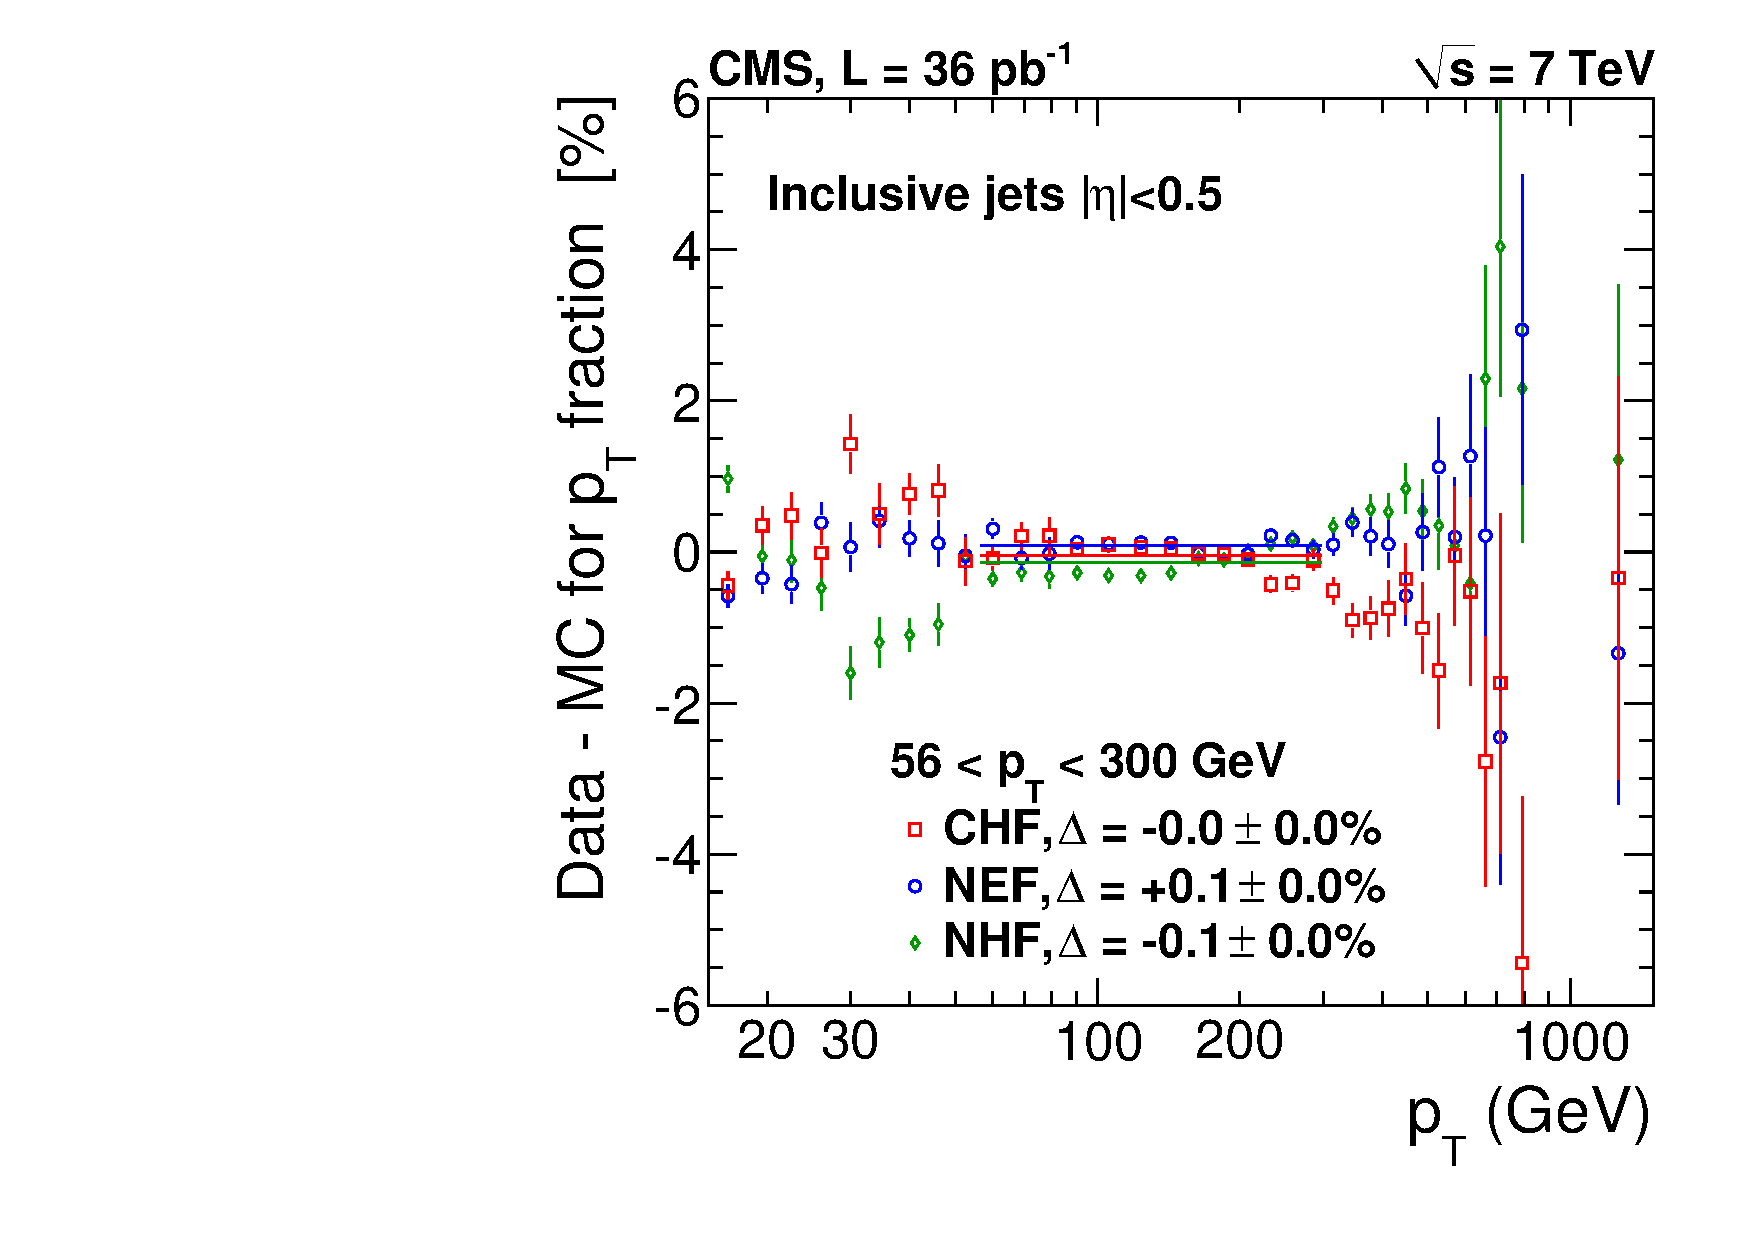
\includegraphics[width=0.45\textwidth]{Figures/JEC/jecChecks_fracDataMinusMC_Rap0.pdf}
    \caption{PF jet composition. Left: energy fraction carried by charged hadrons (CHF), photons (NEF), and neutral hadrons (NHF) as a function of jet \pt in the region $|\eta|<0.5$. The filled histograms and the markers represent the data and the simulation respectively. Right: \pt fraction difference between data and MC.}
    \label{fig:composition}
  \end{center}
\end{figure}

Figure~\ref{fig:composition} (left) shows the fraction of jet energy carried by the various particle types. Charged hadrons, photons, and neutral hadrons carry $\sim 65\%,\,20\%$, and $15\%$ of the jet energy respectively at low jet \pt, as expected from the general properties of the fragmentation process. As the jet \pt increases, charged hadrons become more energetic and more collimated, while the tracking efficiency and momentum resolution worsen. This increases the probability for a charged hadron to leave detectable energy only in the calorimeters and to be classified either as a neutral electromagnetic object (photon) or as a neutral hadron. Therefore, for higher jet \pt, the energy fraction carried by photons and neutral hadrons is increased. The excellent agreement between data and simulation quantified in Fig.~\ref{fig:composition} (right) proves that the simulation can be safely trusted to predict the absolute jet energy response. 

\begin{figure}[ht!]
  \begin{center}
    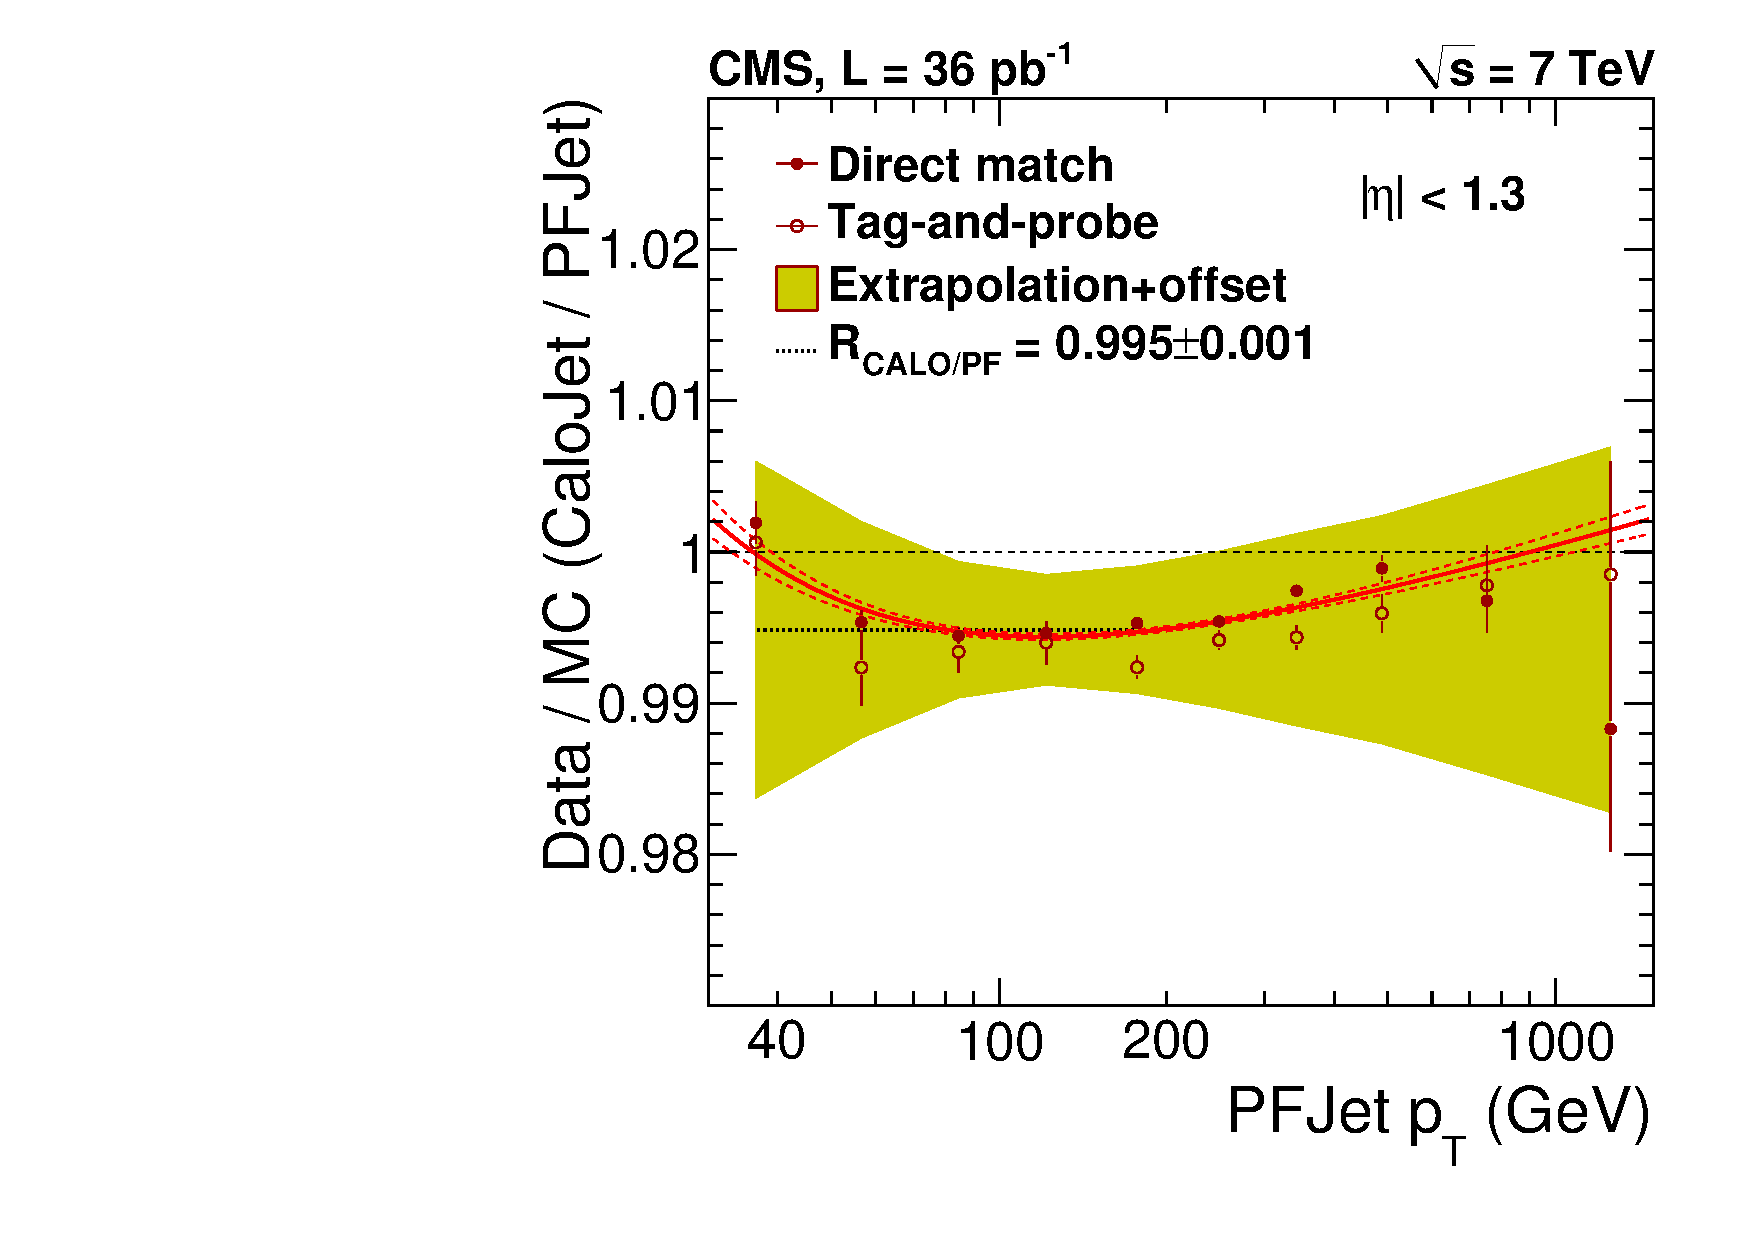
\includegraphics[width=0.45\textwidth]{Figures/JEC/jetmatch013_calopf.pdf}
    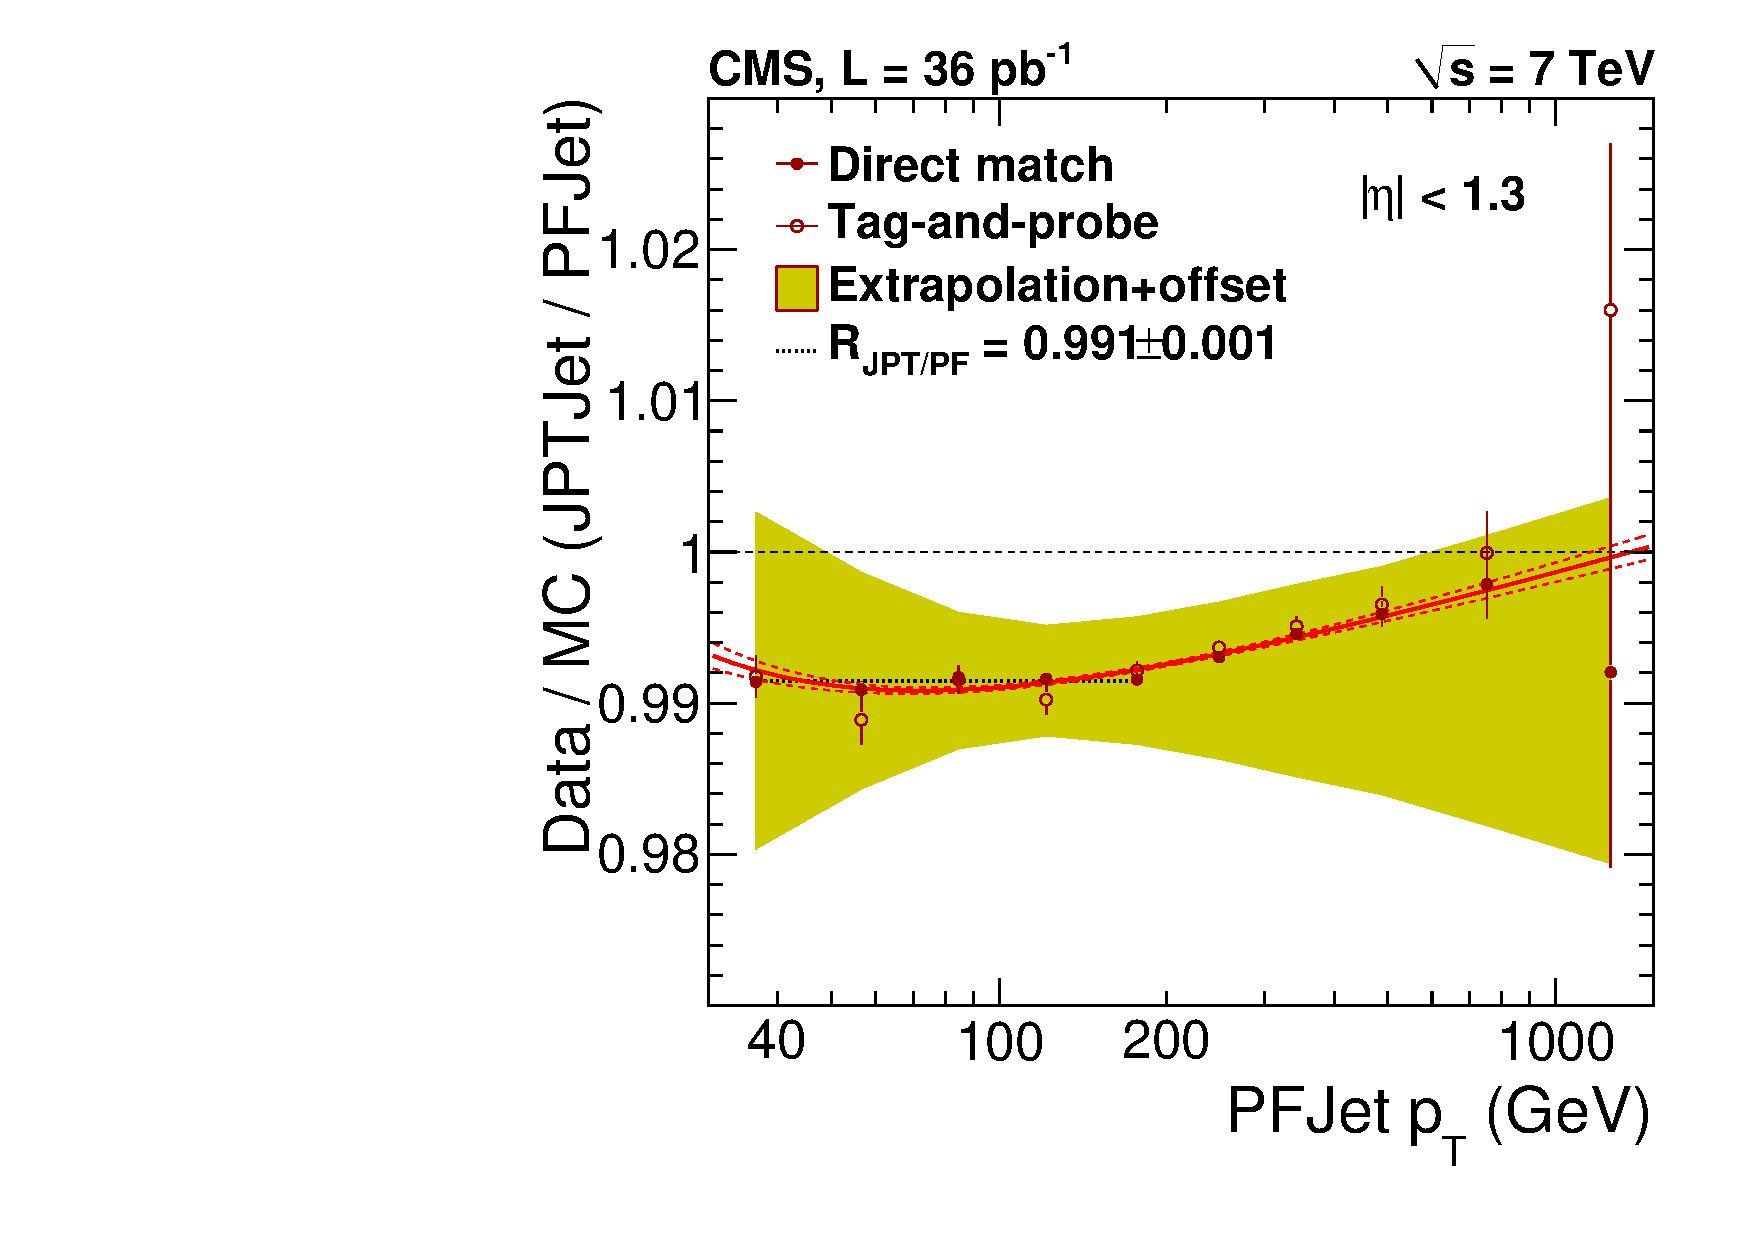
\includegraphics[width=0.45\textwidth]{Figures/JEC/jetmatch013_jptpf.pdf}
    \caption{Left: CALO vs. PF jet \pt response ratio between data and MC simulation. Right: JPT vs. PF jet \pt response ratio between data and MC simulation. The solid circles correspond to direct matching in the $\eta-\phi$ space and the open circles correspond to a tag (PF jet) and probe (CALO/JPT jet) method.}
    \label{fig:caloVsPF}
  \end{center}
\end{figure}

{\bf Jet-by-Jet Matching.} Once the jet energy scale is established for PF jets, the estimated uncertainties are transfered to the other jet types. This is done by direct jet-by-jet comparison between different jet types in the QCD dijet sample. The PF and CALO (JPT) jets are spatially matched in the $\eta,\,\phi$ space by requiring $\DeltaR<0.25$. For the matched jet pairs the relative response of CALO (JPT) jets $\pt^{CALO}/\pt^{PF}$ ($\pt^{JPT}/\pt^{PF}$) is measured as a function of $\pt^{PF}$ (the study is described in detail in Ref.~\cite{JME-10-003}). A cross-check of the direct jet matching is done with a tag-and-probe method in dijet events, with the PF jet being the tag object and the CALO/JPT jets being the probe objects. The results are summarized in Fig.~\ref{fig:caloVsPF} where the response ratio data/MC of the CALO and JPT response relative to the PF jets is shown. The observed disagreement is at the level of $0.5\%$, indicating that the precision of the CALO and JPT calibration is comparable to that of the PF jets. The observed $0.5\%$ level of data/MC disagreement is taken into account as an additional systematic uncertainty for CALO and JPT jets.

\subsubsection{Uncertainty}

As described in the previous sections, the absolute jet energy response is measured in situ for PF jets with the MPF method in $\gamma$/Z+jets events. The systematic uncertainties related to the measurement itself are summarized in Fig.~\ref{fig:jecuncert_mpf}. The estimation of the systematic uncertainty in the kinematic region beyond the reach of the $\gamma$+jets sample is based on the simulation and its sensitivity to the single-particle response and the fragmentation models. In addition, the uncertainty on the $\gamma$ energy scale needs to be taken into account since the jet energy response is measured relative to the $\gamma$ scale. The direct jet-by-jet spatial matching, allows the transfer of the PF jet-energy- scale uncertainty to the other jet types (CALO, JPT). Finally, a flavour uncertainty is assigned from the response differences between the quark and gluon originated jets. These are taken from Fig.~\ref{fig:flavor_herwigpythia} and cover the absolute scale uncertainty in physics samples with a different flavour mixture than the reference QCD multijet sample. 

Figure~\ref{fig:absunc} shows the absolute energy scale uncertainties for the three jet types, combined with the offset correction uncertainty corresponding to the average number of pile-up events in the datasets considered for this paper. The low jet \pt threshold indicates the minimum recommended \pt for each jet type: 30\GeV, 20\GeV, and 10\GeV for CALO, JPT, and PF jets respectively. At low jet \pt the offset uncertainty dominates with significant contribution from the MC truth and jet-by-jet matching residuals. At the intermediate jet \pt, where enough data for the in situ measurements are available, the $\gamma$ energy scale uncertainty dominates. At high jet \pt, the uncertainty due to the MC extrapolation is dominant. Overall, the absolute jet energy scale uncertainty for all jet types is smaller than 2\% for $\pt>40\GeV$. 

\begin{figure}[ht!]
  \begin{center}
    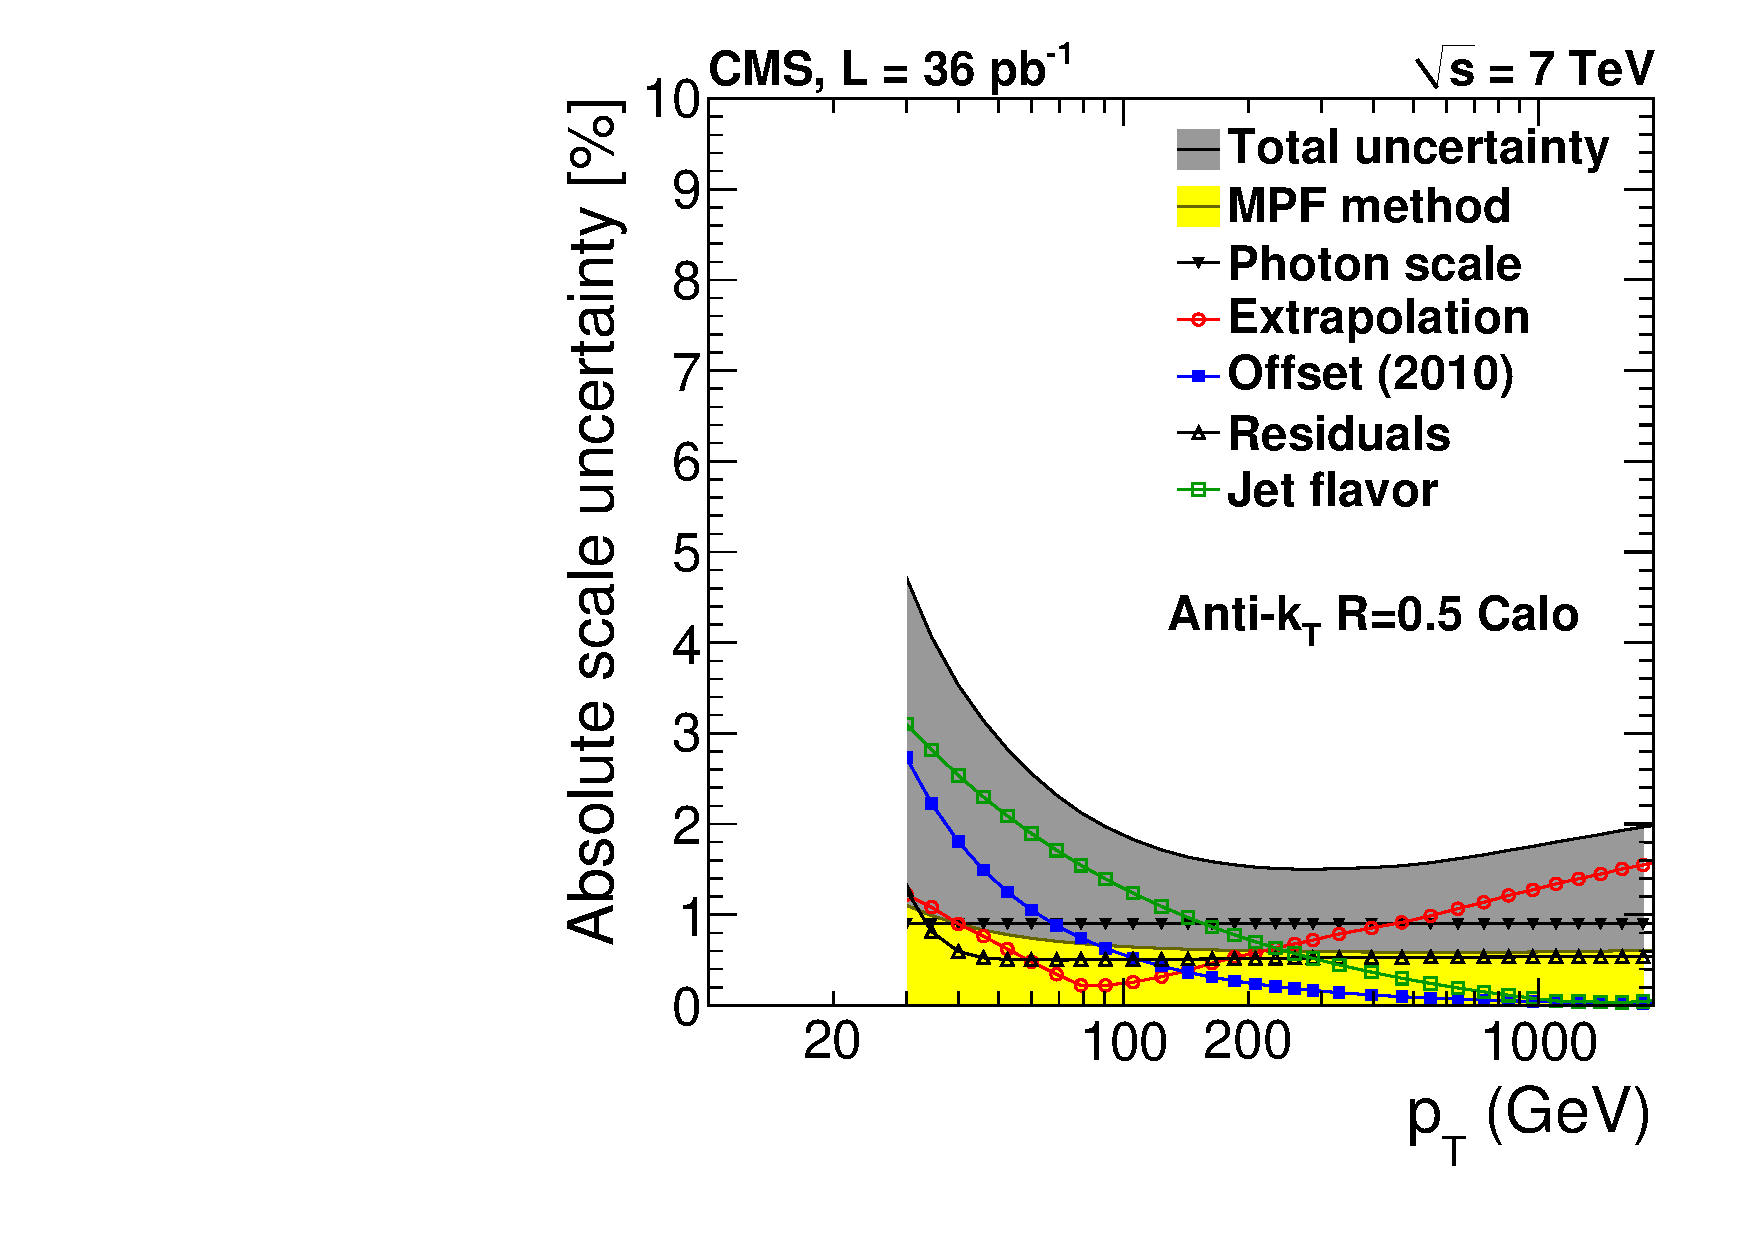
\includegraphics[width=0.45\textwidth]{Figures/JEC/JECUncert_AK5_summary}
    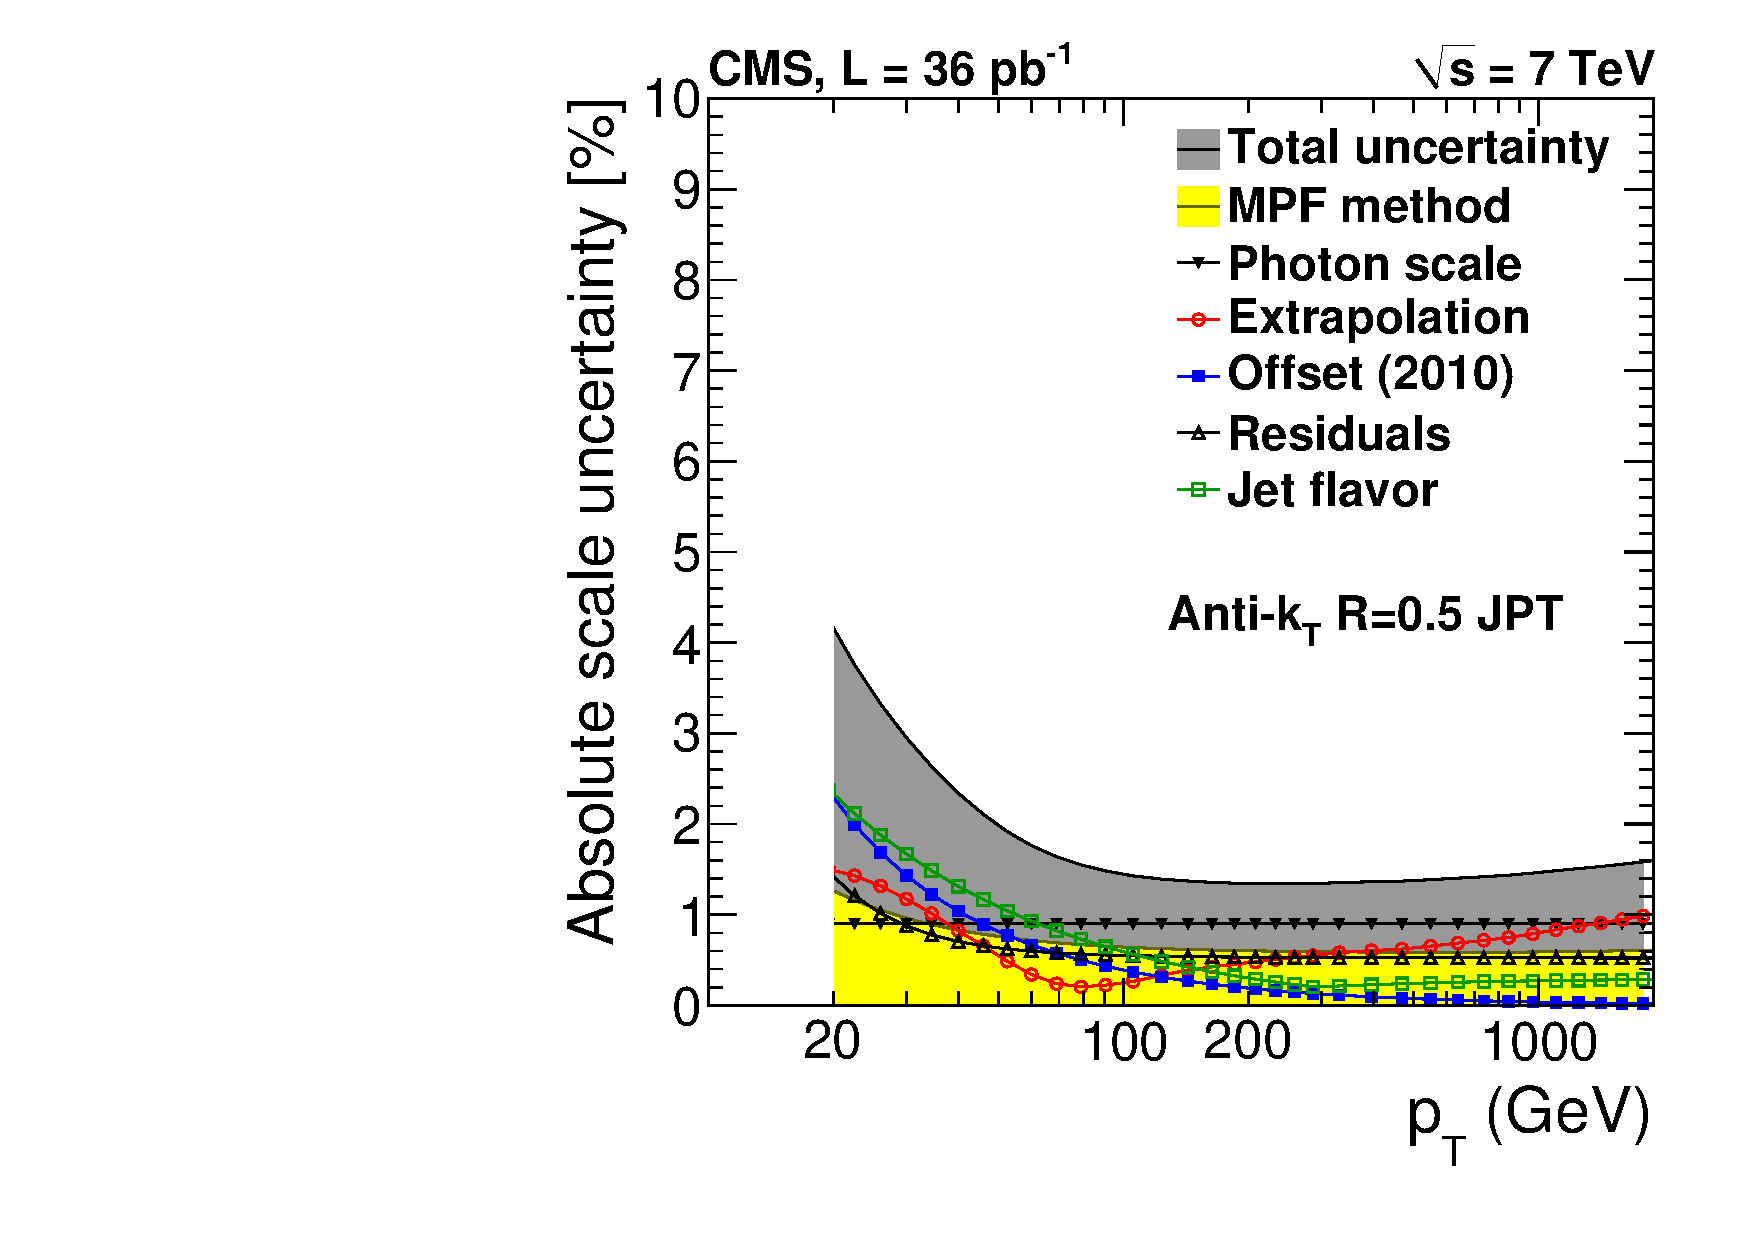
\includegraphics[width=0.45\textwidth]{Figures/JEC/JECUncert_JPTAK5_summary}
    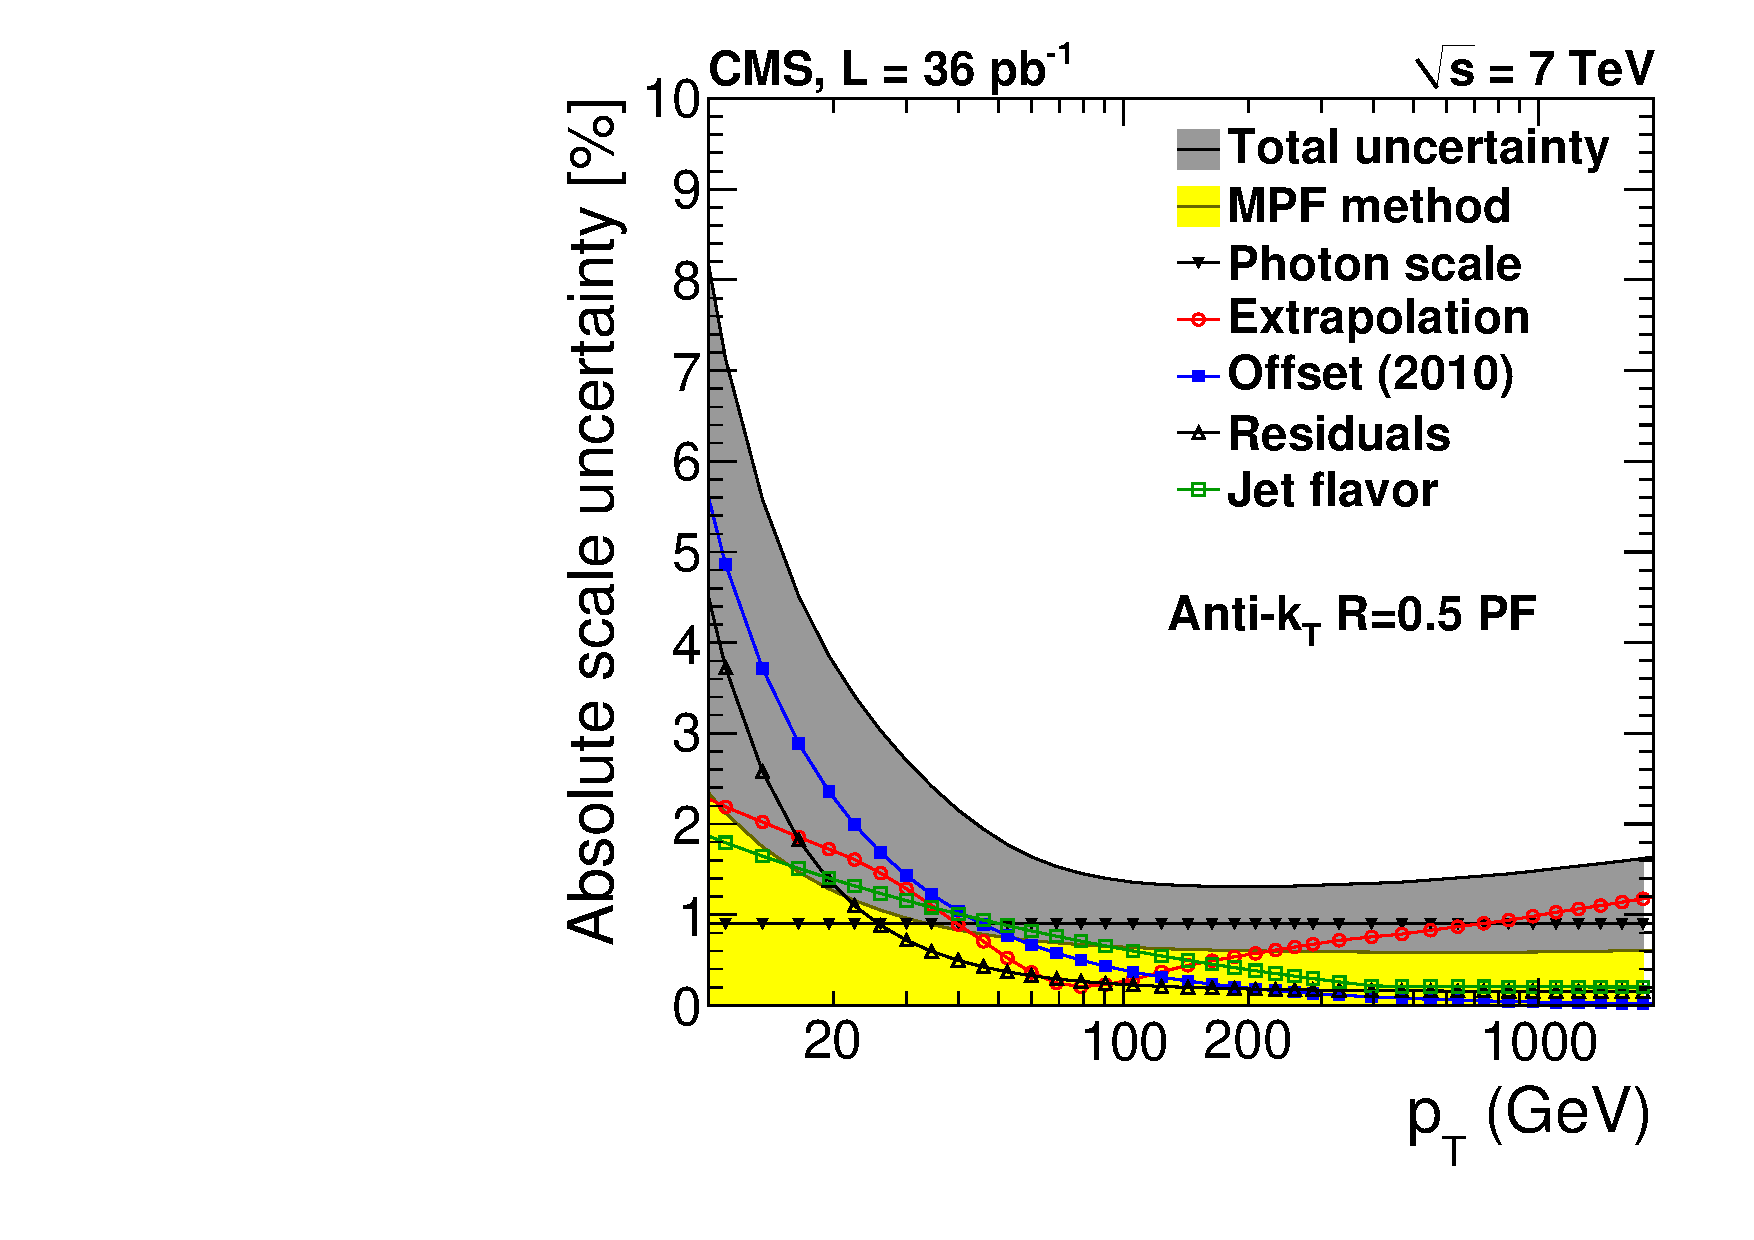
\includegraphics[width=0.45\textwidth]{Figures/JEC/JECUncert_PFAK5_summary}
    \caption{Absolute jet energy scale uncertainty as a function of jet \pt for CALO, JPT and PF jets respectively.}
    \label{fig:absunc}
  \end{center}
\end{figure}

\clearpage
